\chapter{Systèmes d'équations différentielles ordinaires} \label{sys:chapter}

%%%%%%%%%%%%%%%%%%%%%%%%%%%%%%%%%%%%%%%%%%%%%%%%%%%%%%%%%%%%%%%%%%%%%%%%%%%%%%

\section{Introduction aux systèmes d'équations différentielles ordinaires} \label{sec:introtosys}

%\sectionnotes{Lectures supplémentaires : \EPref{\S4.1 dans %\cite{EP}}\BDref{ et
%\S7.1 dans \cite{BD}}}

\subsection{Systèmes différentiels}

Un problème n'a pas toujours qu'une seule variable dépendante et qu'une seule équation. Comme on le verra, des systèmes peuvent être composés de plusieurs équations et de plusieurs variables dépendantes même s'il n'y a qu'une seule équation au départ.

S'il y a plusieurs variables dépendantes, $y_1$, $y_2$, \ldots, $y_n$,
alors
il peut y avoir une équation différentielle comprenant toutes ces variables et leurs dérivées par rapport à une variable indépendante $x$.
Par exemple, $y_1'' = f(y_1',y_2',y_1,y_2,x)$.
Généralement, lorsqu'il y a deux variables dépendantes, il y a deux équations telles que
\begin{align*}
y_1'' & = f_1(y_1',y_2',y_1,y_2,x) , \\
y_2'' & = f_2(y_1',y_2',y_1,y_2,x)
\end{align*}
pour des fonctions $f_1$ et $f_2$. On appelle ça un
\emph{\myindex{système d'équations différentielles}}.
De façon plus précise, l'équation précédente est un \emph{\myindex{système d'EDO du second ordre}}
étant donné la présence d'une dérivée du second ordre. Le système
\begin{align*}
x_1' & = g_1(x_1,x_2,x_3,t) , \\
x_2' & = g_2(x_1,x_2,x_3,t) , \\
x_3' & = g_3(x_1,x_2,x_3,t) 
\end{align*}
est du \emph{\myindex{premier ordre}}, où $x_1,x_2$ et $x_3$ sont les variables dépendantes et où $t$ est la variable indépendante.

La terminologie des systèmes est essentiellement la même que pour les équations simples. Pour le système précédent, une 
\emph{solution}\index{solution pour un système}
est un ensemble de trois fonctions $x_1(t)$, $x_2(t)$, $x_3(t)$ telles que
\begin{align*}
x_1'(t) &= g_1\bigl(x_1(t),x_2(t),x_3(t),t\bigr) , \\
x_2'(t) &= g_2\bigl(x_1(t),x_2(t),x_3(t),t\bigr) , \\
x_3'(t) &= g_3\bigl(x_1(t),x_2(t),x_3(t),t\bigr) .
\end{align*}

Généralement, il y a aussi une
\emph{condition initiale}\index{condition initiale pour un système}. Comme dans le cas des équations simples, on précise $x_1$, $x_2$ et $x_3$ pour un $t$ fixe.
Par exemple, $x_1(0) = a_1$, $x_2(0) = a_2$ et $x_3(0) = a_3$, où $a_1$, $a_2$ et $a_3$ sont des constantes quelconques. Pour le système du second ordre, on préciserait également les premières dérivées en un point. Si l'on trouve une solution avec des constantes et que, en résolvant celles-ci, on trouve une solution pour toute condition initiale, on appelle cette solution la \emph{solution générale}\index{solution générale d'un système}.
Examinons un exemple simple.

\begin{example}
Il est parfois facile de trouver la solution en résolvant un système pour une variable puis pour la seconde. Prenons le système du premier ordre
\begin{align*}
y_1' & = y_1 , \\
y_2' & = y_1 - y_2 ,
\end{align*}
où $y_1$ et $y_2$ sont les variables dépendantes et où $x$ est la variable indépendante. Considérons les conditions initiales 
$y_1(0) = 1$ et $y_2(0) = 2$.

On remarque que $y_1 = C_1 e^x$ est la solution générale de la première équation. En substituant ensuite ce $y_1$ dans la seconde équation, on obtient $y_2' = C_1e^x - y_2$, qui est une équation linéaire du premier ordre facilement résoluble pour $y_2$. Avec la méthode du facteur intégrant, on obtient
\begin{equation*}
e^x y_2 = \frac{C_1}{2}e^{2x} + C_2
\end{equation*}
ou $y_2 = \frac{C_1}{2}e^{x} + C_2e^{-x}$. La solution générale du système est donc :
\begin{equation*}
y_1 = C_1 e^x , \qquad
y_2 = \frac{C_1}{2}e^{x} + C_2e^{-x} .
\end{equation*}
On résout le système pour $C_1$ et $C_2$ pour les conditions initiales. On substitue $x=0$ et l'on trouve que 
$C_1=1$ et $C_2=\nicefrac{3}{2}$. Alors, la solution est
$y_1 = e^x$ et
$y_2 = (\nicefrac{1}{2}) e^x + (\nicefrac{3}{2}) e^{-x}$.
\end{example}

En général, on ne peut pas résoudre chaque variable séparément comme dans l'exemple précédent, et il faudra résoudre toutes les variables en même temps. Même si l'on ne peut pas toujours résoudre le système pour une variable et ensuite pour la suivante, on essaiera de tirer profit au maximum de cette technique. D'une certaine façon, on résoudra plusieurs équations simples et l'on regroupera les solutions. Ne nous préoccupons pas encore de la façon de résoudre les systèmes d'équations.

Considérons principalement les \emph{\myindex{systèmes linéaires}}. L'exemple précédent est un \emph{\myindex{système linéaire du premier ordre}}, car les variables dépendantes ou leurs dérivées n'apparaissent pas dans des fonctions non linéaires ou à des puissances supérieures à un ($x$, $y$, $x'$ et $y'$ constantes, et les fonctions de $t$
peuvent être présentes, mais pas $xy$ ni ${(y')}^2$ ni $x^3$). Voici un exemple plus complexe de système linéaire :
\begin{align*}
y_1'' &= e^t y_1' + t^2 y_1 + 5 y_2 + \sin(t), \\
y_2'' &= t y_1'-y_2' + 2 y_1 + \cos(t).
\end{align*}

\subsection{Applications}

Voici quelques applications simples de systèmes différentiels et la manière de mettre en place les équations.

\begin{example} \label{sintro:closedbrine-example}
Tout d'abord, examinons des réservoirs de solution saline, mais, cette fois-ci, l'eau circule de l'un à l'autre, et vice versa. Considérons que les réservoirs sont mélangés uniformément.

\begin{myfig}
\capstart
\inputpdft{lin-tank-sys}
\caption{Système fermé de deux réservoirs de solution saline.\label{sintro:closedbrine}}
\end{myfig}

Supposons que nous avons deux réservoirs contenant un volume de $V$ litres d'eau salée. Le premier réservoir contient $x_1$ grammes de sel, et le second, $x_2$ grammes. La solution est parfaitement mélangée et s'écoule d'un réservoir à l'autre à la vitesse de $r$ litres par seconde. Voir la \figurevref{sintro:closedbrine}.

Le taux de variation de $x_1$,
c'est-à-dire $x_1'$, est la différence entre les débits d'entrée et de sortie. Le débit entrant correspond à la densité du sel dans le réservoir 2 ($\frac{x_2}{V}$) multipliée par le débit $r$.
Le débit sortant correspond à la densité du sel dans le réservoir 1 ($\frac{x_1}{V}$) multipliée par le débit $r$.
En d'autres termes, on a
\begin{equation*}
x_1' = \frac{x_2}{V} r - \frac{x_1}{V} r =
\frac{r}{V} x_2 - \frac{r}{V} x_1 = \frac{r}{V} (x_2-x_1).
\end{equation*}
De la même façon, on trouve le taux de variation de $x_2'$ quand les rôles de $x_1$ et $x_2$
sont inversés. En résumé, le système d'EDO de ce problème est
\begin{align*}
x_1' & = \frac{r}{V} (x_2-x_1), \\
x_2' & = \frac{r}{V} (x_1-x_2).
\end{align*}
Ici, on ne peut pas résoudre le système séparément pour $x_1$ ou $x_2$. On doit simultanément le résoudre pour $x_1$ et $x_2$, ce qui est évident étant donné que la quantité de sel dans un réservoir affecte celle dans l'autre. On ne peut déterminer $x_1$ sans $x_2$, et vice versa.

On ne sait pas encore comment trouver toutes les solutions, mais on peut au moins en trouver certaines de façon intuitive. Supposons que nous savons que les réservoirs contiennent la même quantité de sel au départ. On a donc la condition initiale $x_1(0)=x_2(0) = C$. Dans ce cas, la quantité de sel qui sort de chaque réservoir est la même, alors les concentrations ne changent pas. En d'autres termes, $x_1 = C$ et $x_2 = C$ (les fonctions constantes) est une solution : $x_1' = x_2' = 0$ et
$x_2-x_1 = x_1-x_2 = 0$, alors les équations sont satisfaites.

Réfléchissons encore un peu avant de résoudre le système. Supposons des conditions initiales $x_1(0) = A$ et $x_2(0) = B$, pour deux constantes différentes $A$ et $B$. On a un système fermé, alors la quantité totale de sel est constante. Donc, $x_1+x_2$ est constant et égal à $A+B$.
Si $A$ est plus grande que $B$, il y aura plus de sel qui sort du premier réservoir qu'il y en entre. Éventuellement, après une longue période, la quantité de sel dans chaque réservoir sera égale. Donc, la solution de $x_1$ et $x_2$ tend vers $\frac{A+B}{2}$. Vous découvrirez que c'est vrai quand vous aurez appris à résoudre des systèmes différentiels.
\end{example}

\begin{example} \label{sintro:carts-example}
Étudions un exemple du second ordre. Reprenons le montage avec une masse et un ressort, mais, cette fois-ci, considérons deux masses.

\begin{mywrapfigsimp}{2.0in}{2.3in}
\noindent
\inputpdft{cartsfig}
\end{mywrapfigsimp}
On a un ressort avec une constante $k$ et deux masses $m_1$
et $m_2$. Imaginez les masses comme des chariots qui se déplacent sans friction le long d'une voie linéaire. La variable $x_1$ représente le déplacement du premier chariot, et $x_2$, le déplacement du second. Les deux chariots reposent sans tension dans le ressort, et l'on marque la position des deux chariots qu'on appelle les positions zéro. Alors, $x_1$ indique la distance du premier chariot par rapport à sa position zéro, et $x_2$ fait la même chose pour le second. La force exercée par le ressort sur le premier chariot est
$k(x_2-x_1)$ étant donné que 
$x_2-x_1$ représente l'étirement (ou la compression) du ressort par rapport à la position de repos. La force exercée sur le second chariot est l'inverse, donc la même avec un signe négatif. La 
\myindex{deuxième loi de Newton} stipule que la force est égale à la masse multipliée par l'accélération. Le système d'équations est donc
\begin{align*}
m_1 x_1'' & = k(x_2-x_1) , \\
m_2 x_2'' & = - k(x_2-x_1) .
\end{align*}

Encore une fois, on ne peut le résoudre pour les variables $x_1$ et $x_2$ séparément. Il est clair qu'on doit résoudre le système pour $x_1$ et $x_2$ en même temps, car les déplacements des deux chariots sont interreliés.
\end{example}

\subsection{Passage au premier ordre}

Avant de parler de la façon de traiter des systèmes différentiels, notons que, dans un certain sens, nous pouvons ne considérer que les systèmes du premier ordre. Prenons une équation différentielle de $n^{\text{e}}$ ordre :
\begin{equation*}
y^{(n)} = F(y^{(n-1)},\ldots,y',y,x) .
\end{equation*}
On définit de nouvelles variables $u_1, u_2, \ldots, u_n$ et l'on écrit le système :
\begin{align*}
u_1' & = u_2 , \\
u_2' & = u_3 , \\
& ~\, \vdots \\
u_{n-1}' & = u_n , \\
u_n' & = F(u_n,u_{n-1},\ldots,u_2,u_1,x) .
\end{align*}
On résout ce système pour $u_1$, $u_2$, \ldots, $u_n$. Après avoir trouvé la solution pour les $u$,
on peut oublier $u_2$ à $u_n$ et garder $y = u_1$.
Ce $y$ résout l'équation d'origine.

\begin{example}
Prenons $x''' = 2x''+ 8x' + x + t$. Si l'on admet que $u_1 = x$, $u_2 = x'$ et $u_3
= x''$, on trouve le système :
\begin{equation*}
u_1' = u_2, \qquad u_2' = u_3, \qquad u_3' = 2u_3 + 8u_2 + u_1 + t .
\end{equation*}
\end{example}

On peut suivre une démarche similaire pour un système d'équations différentielles d'ordre supérieur. Par exemple, un système de $k$ équations différentielles avec $k$
inconnues, toutes d'ordre $n$, peut être ramené à un système du premier ordre de 
$n \times k$
équations et de $n \times k$ inconnues.

\begin{example}
Reprenons l'exemple des chariots,
\begin{equation*}
m_1 x_1'' = k(x_2-x_1), \qquad m_2 x_2'' = - k(x_2-x_1) .
\end{equation*}
Admettons que $u_1 = x_1$, $u_2 = x_1'$, 
$u_3 = x_2$ et $u_4 = x_2'$. Le système du second ordre devient le système du premier ordre :
\begin{equation*}
u_1' = u_2, \qquad
m_1 u_2' = k(u_3-u_1), \qquad
u_3' = u_4, \qquad
m_2 u_4' = - k(u_3-u_1) .
\end{equation*}
\end{example}

\begin{example}
Le principe fonctionne dans les deux sens. Prenons le système
\begin{equation*}
x' = 2y-x , \qquad
y' = x, 
\end{equation*}
où la variable indépendante est $t$. On désire le résoudre pour les conditions initiales $x(0) = 1$ et $y(0) =0$.

Si l'on dérive la seconde équation, on obtient
$y''=x'$. On sait ce que représente $x'$ en fonction de $x$ et $y$, et l'on sait que $x=y'$. Alors,
\begin{equation*}
y'' = x' = 2y-x = 2y-y' .
\end{equation*}
On a maintenant l'équation $y''+y'-2y = 0$. On sait comment résoudre cette équation et l'on trouve que $y = C_1 e^{-2t} + C_2 e^t$. Maintenant qu'on a $y$,
on utilise l'équation $y' = x$ pour trouver $x$ :
\begin{equation*}
x = y' = -2 C_1 e^{-2t} + C_2 e^t .
\end{equation*}
On résout pour les conditions initiales $1 = x(0) = -2 C_1 + C_2$
et $0 = y(0) = C_1 + C_2$. Ainsi, $C_1 = -C_2$ et $1 = 3C_2$.
Donc, $C_1 = \nicefrac{-1}{3}$ et $C_2 = \nicefrac{1}{3}$. La solution est
\begin{equation*}
x = \frac{2e^{-2t} + e^t}{3} ,\qquad
y = \frac{-e^{-2t} + e^t}{3} .
\end{equation*}
\end{example}

\begin{exercise}
Remplacez les termes et vérifiez que la solution est bonne.
\end{exercise}

L'aller-retour entre les systèmes et les équations d'ordre supérieur est utile pour d'autres raisons. Par exemple, le logiciel utilisé pour résoudre numériquement les EDO (approximation) traite généralement les systèmes du premier ordre. Pour l'utiliser, on doit donc prendre l'EDO à résoudre et la ramener à un système du premier ordre. En réalité, c'est assez simple d'adapter le code informatique pour la méthode d'Euler ou celle de Runge-Kutta pour les équations du premier ordre afin de résoudre ces systèmes. Il suffit alors de traiter la variable dépendante comme un vecteur au lieu d'un nombre. La syntaxe est semblable pour la plupart des langages informatiques mathématiques.

%In fact, this is what IODE was doing when you had it solve a second order
%equation numerically in the IODE Project III if you have done that project.

\subsection{Systèmes autonomes et champs de vecteurs}

Un système où les équations ne dépendent pas de la variable indépendante se nomme un \emph{\myindex{système autonome}}. Par exemple, le système $x'=2y-x$, $y'=x$ est autonome, car $t$ est la variable indépendante, mais elle n'apparaît pas dans les équations.

Pour les systèmes autonomes, on peut utiliser un
\emph{\myindex{champ de vecteurs associé au système}} ou \emph{\myindex{champ vectoriel}},
qui est un graphe semblable au champ de directions, mais, au lieu de donner une pente à chaque point, on donne une direction (et une amplitude). L'exemple précédent, $x' = 2y-x$, $y' = x$, indique que, au point $(x,y)$, la direction dans laquelle on doit se déplacer pour satisfaire aux équations devrait correspondre à la direction du vecteur $( 2y-x, x )$
à une vitesse égale à l'amplitude de ce vecteur. On dessine donc le vecteur $(2y-x,x)$ au point $(x,y)$ et l'on répète pour plusieurs points sur le plan $xy$.
Par exemple, au point $(1,2)$, on dessine le vecteur
$\bigl(2(2)-1,1\bigr) = (3,1)$,
qui pointe vers la droite et légèrement vers le haut, alors que, au point $(2,1)$, on dessine le vecteur $\bigl(2(1)-2,2\bigr) = (0,2)$,
qui pointe directement vers le haut.
Lorsqu'on trace les vecteurs, on réduit leur taille afin de pouvoir en placer plusieurs sur le même champ de vecteurs. On s'intéresse principalement à leur direction et à leur taille relative. Voir la
\figureref{sintro-vectorfield:fig}.

On peut dessiner une trajectoire de la solution dans le plan. Supposons que $x = f(t)$ et que $y=g(t)$ est la solution. Nous choisissons un intervalle de $t$ (disons $0 \leq t \leq 2$ pour l'exemple) et nous traçons trace tous les points
$\bigl(f(t),g(t)\bigr)$ pour la plage $t$ sélectionnée. L'image obtenue est appelée \emph{\myindex{portrait de phase}}
(ou \emph{\myindex{portrait de phase du plan}}).
La courbe particulière obtenue est appelée \emph{\myindex{trajectoire}} ou \emph{\myindex{courbe de solution}}.
La \figureref{sintro-vectorfield-sol:fig} donne un exemple de tracé.
Sur le graphe, la solution commence au point $(1,0)$ et se déplace le long du champ vectoriel sur une distance de deux unités de $t$. Ce système a été résolu avec précision, alors on calcule $x(2)$ et $y(2)$ pour trouver
$x(2) \approx 2.475$ et $y(2) \approx 2.457$. Ce point correspond à l'extrémité supérieure droite de la courbe de solution tracée sur le graphe.

\begin{myfig}
\parbox[t]{3.0in}{
 \capstart
 \diffyincludegraphics{width=3.0in}{width=4.5in}{sintro-vectorfield}
 \caption{Portrait de phase pour $x' = 2y-x$, $y' = x$.%
 \label{sintro-vectorfield:fig}}
}
\quad
\parbox[t]{3.0in}{
 \capstart
 \diffyincludegraphics{width=3.0in}{width=4.5in}{sintro-vectorfield-sol}
 \caption{Portrait de phase pour $x' = 2y-x$, $y' = x$, avec la trajectoire de la solution commençant au point $(1,0)$
 pour $0 \leq t \leq 2$.%
 \label{sintro-vectorfield-sol:fig}}
}
\end{myfig}


Observez la similitude avec les diagrammes pour les systèmes autonomes à une dimension. Toutefois, remarquez comment les choses se compliquent quand on n'ajoute qu'une autre dimension.
On peut tracer des portraits de phase et des trajectoires dans le plan $xy$
même si le système n'est pas autonome. Cependant, dans ce cas, on ne peut pas dessiner de champ de vecteurs étant donné que le champ se modifie à mesure que $t$ change. Chaque $t$ donne un champ vectoriel différent.

\subsection{Théorème de Picard}

Avant d'aller plus loin, mentionnons que le théorème de Picard sur l'existence et l'unicité est toujours valable pour les systèmes d'EDO\@. Rappelons ce théorème pour les systèmes différentiels. Un système du premier ordre générique prend la forme
\begin{equation} \label{eq:general-system}
\begin{aligned}
x_1' & = F_1(x_1,x_2,\ldots,x_n,t) , \\
x_2' & = F_2(x_1,x_2,\ldots,x_n,t) , \\
& \vdots \\
x_n' & = F_n(x_1,x_2,\ldots,x_n,t) .
\end{aligned}
\end{equation}

\begin{theorem}[Théorème de Picard sur l'existence et l'unicité des systèmes]%
\label{sys:picardthm}%
\index{existence and uniqueness for systems}\index{Picard's theorem}
Si, pour chaque $j=1,2,\ldots,n$ et pour chaque
$k = 1,2,\ldots,n$,
chaque $F_j$ est continue et que la dérivée
$\frac{\partial F_j}{\partial x_k}$ existe et est continue dans une région contenant $(x_1^0,x_2^0,\ldots,x_n^0,t^0)$, alors la solution à 
\eqref{eq:general-system}
soumise aux conditions initiales
$x_1(t^0) = x_1^0$,
$x_2(t^0) = x_2^0$, \ldots,
$x_n(t^0) = x_n^0$
existe (du moins pour un petit intervalle autour de $t$) et est unique.
\end{theorem}

Plus simplement, une solution unique existe pour toute condition initiale si le système est raisonnable ($F_j$ et ses dérivées partielles selon $x$ sont continues). Quant aux équations simples, il se peut qu'il n'y ait pas de solution pour chaque temps $t$, mais il peut y en avoir pour au moins de courtes périodes.
Comme on peut transformer n'importe quelle EDO d'ordre $n$ en un  système du premier ordre, ce théorème permet également l'existence et l'unicité des solutions pour des équations d'ordre supérieur qui n'ont pas encore été énoncées explicitement.

\subsection{Exercices}

\begin{exercise}
Trouvez la solution générale de $x_1' = x_2 - x_1 + t$, $x_2' = x_2$.
\end{exercise}

\begin{exercise}
Trouvez la solution générale de $x_1' = 3 x_1 - x_2 + e^t$, $x_2' = x_1$.
\end{exercise}

\begin{exercise}
Écrivez $ay'' + by' + cy = f(x)$
sous forme de système d'EDO de premier ordre.
\end{exercise}

\begin{exercise}
Écrivez $x'' + y^2 y' - x^3 = \sin(t)$, 
$y'' + {(x'+y')}^2 -x = 0$ sous forme de système d'EDO de premier ordre.
\end{exercise}

\begin{exercise}
Supposons que deux masses sur des chariots se déplaçant sur une surface sans friction soient aux positions $x_1$ et $x_2$ comme dans l'\exampleref{sintro:carts-example}.
Supposons qu'une fusée applique une force $F$ de direction positive sur le chariot
$x_1$. Configurez le système d'équations différentielles.
\end{exercise}

\begin{exercise}
Supposons que des réservoirs soient disposés comme dans l'\exampleref{sintro:closedbrine-example} et que les deux aient un volume de départ $V$,
mais maintenant, le débit du réservoir 1 vers le réservoir 2 est $r_1$ et le débit du réservoir 2 vers le réservoir 1 est $r_2$. Dans ce cas, les volumes changeront. Configurez le système d'équations différentielles.
\end{exercise}

\setcounter{exercise}{100}

\begin{exercise}
Trouvez la solution générale de $y_1' = 3 y_1$, $y_2' = y_1 + y_2$,
$y_3' = y_1 + y_3$.
\end{exercise}
\exsol{%
$y_1 = C_1 e^{3x}$,
$y_2 = y(x) = C_2 e^x+ \frac{C_1}{2} e^{3 x}$,
$y_3 = y(x) = C_3 e^x+ \frac{C_1}{2} e^{3 x}$
}

\begin{exercise}
Résolvez $y'=2x$, $x'=x+y$, $x(0)=1$, $y(0)=3$.
\end{exercise}
\exsol{%
$x=\frac{5}{3} e^{2t} - \frac{2}{3} e^{-t}$,
$y=\frac{5}{3} e^{2t} + \frac{4}{3} e^{-t}$
}

\begin{exercise}
Écrivez $x''' = x+t$ sous forme de  système du premier ordre.
\end{exercise}
\exsol{%
$x_1' = x_2$,
$x_2' = x_3$,
$x_3' = x_1+t$
}

\begin{exercise}
Écrivez $y_1'' + y_1 + y_2 = t$, 
$y_2'' + y_1 - y_2 = t^2$ sous forme de  système du premier ordre.
\end{exercise}
\exsol{%
$y_3' + y_1 + y_2 = t$, 
$y_4' + y_1 - y_2 = t^2$,
$y_1' = y_3$,
$y_2' = y_4$
}

\begin{exercise}
Supposons que deux masses sur des chariots qui se déplacent sur une surface sans friction soient aux positions $x_1$ et $x_2$ comme dans l'\exampleref{sintro:carts-example}.
Supposons que la position initiale soit $x_1(0)=x_2(0)=0$ et que la vitesse initiale soit $x_1'(0) = x_2'(0) = a$ pour un nombre quelconque $a$.
Utilisez votre intuition pour résoudre le système différentiel et expliquez votre raisonnement.
\end{exercise}
\exsol{%
$x_1 = x_2 = at$. Explanation of the intuition is left to reader.
}

\begin{exercise}
Supposons que des réservoirs soient disposés comme dans l'\exampleref{sintro:closedbrine-example}, mais cette fois, de l'eau propre s'écoule à un débit de $s$ litres par seconde vers le réservoir 1 et une solution saline s'écoule dans le réservoir 2 et dans les égouts avec un même débit de $s$ litres par seconde.
\begin{tasks}
\task Dessinez le schéma.
\task Configurez le système d'équations différentielles.
\task De façon intuitive, qu'arrive-t-il lorsque $t$ tend vers l'infini? Expliquez.
\end{tasks}
\end{exercise}
\exsol{%
a) Laissé au lecteur.
\quad b) 
$x_1' = \frac{r}{V} (x_2-x_1)$,
$x_2' = \frac{r}{V} x_1- \frac{r-s}{V}x_2$.
\quad c) Lorsque $t$ tend vers l'infini, chacun de $x_1$ et $x_2$ tendent vers zéro, et le lecteur peut compléter l'explication.
}

%%%%%%%%%%%%%%%%%%%%%%%%%%%%%%%%%%%%%%%%%%%%%%%%%%%%%%%%%%%%%%%%%%%%%%%%%%%%%%

\sectionnewpage
\section{Matrices et systèmes linéaires} \label{sec:matrix}

\sectionnotes{Lecture supplémentaire dans l' 
%\EPref{première partie de \S5.1 dans \cite{EP}}\BDref{,
%\S7.2 et \S7.3 dans \cite{BD}}, voir aussi 
\appendixref{linalg:appendix}.}

\subsection{Matrices et vecteurs}

Avant de parler de systèmes linéaires d'EDO, il faut parler de matrices, alors une révision rapide s'impose. Une \emph{\myindex{matrice}} est un tableau de $m
\times n$ nombres ($m$ lignes et $n$ colonnes). Par exemple, on écrit une matrice $3 \times 5$ comme suit :
\begin{equation*}
A = 
\begin{bmatrix}
a_{11} & a_{12} & a_{13} & a_{14} & a_{15} \\
a_{21} & a_{22} & a_{23} & a_{24} & a_{25} \\
a_{31} & a_{32} & a_{33} & a_{34} & a_{35}
\end{bmatrix} .
\end{equation*}
On appelle \emph{éléments}\index{element of a matrix}
ou \emph{composantes}\index{entry of a matrix} les nombres $a_{ij}$.

Un \emph{\myindex{vecteur}} désigne généralement un
\emph{\myindex{vecteur colonne}}, c'est-à-dire une matrice $m \times 1$.
Lorsqu'on parle d'un \emph{\myindex{vecteur ligne}}, on le précise (un vecteur ligne est une matrice $1 \times n$).
On désigne généralement les matrices par des lettres majuscules, et les vecteurs par des minuscules avec une flèche au-dessus, comme $\vec{x}$ ou $\vec{b}$. Un vecteur ne comprenant que des 0 s'écrit $\vec{0}$.

Définissons quelques opérations sur les matrices. Comme on veut que les matrices $1 \times 1$ se comportent comme des nombres, les opérations doivent être compatibles avec ce principe.

Pour commencer, on peut multiplier\index{scalar multiplication} une matrice par un \emph{\myindex{scalaire}} (un nombre).
On multiplie simplement chaque élément de la matrice par le scalaire. Par exemple,
\begin{equation*}
2
\begin{bmatrix}
1 & 2 & 3 \\
4 & 5 & 6
\end{bmatrix} =
\begin{bmatrix}
2 & 4 & 6 \\
8 & 10 & 12
\end{bmatrix} .
\end{equation*}
L'addition\index{addition of matrices} de matrices est aussi simple. On additionne élément par élément. Par exemple,
\begin{equation*}
\begin{bmatrix}
1 & 2 & 3 \\
4 & 5 & 6
\end{bmatrix} +
\begin{bmatrix}
1 & 1 & -1 \\
0 & 2 & 4
\end{bmatrix}
=
\begin{bmatrix}
2 & 3 & 2 \\
4 & 7 & 10
\end{bmatrix} .
\end{equation*}
On ne peut additionner que deux matrices de même taille.

Si l'on désigne par 0 une matrice dont tous les éléments sont nuls, par
$c$ et $d$ des scalaires, et par $A$, $B$ et $C$ des matrices, on obtient les règles suivantes :
\begin{align*}
A + 0 & = A = 0 + A , \\
A + B & = B + A , \\
(A + B) + C & = A + (B + C) , \\
c(A+B) & = cA+cB, \\
(c+d)A & = cA + dA.
\end{align*}

La \emph{\myindex{transposition}} est une autre opération matricielle utile. Cette opération intervertit simplement les lignes et les colonnes d'une matrice. La transposition de $A$ est notée $A^T$. Par exemple,
\begin{equation*}
\begin{bmatrix}
1 & 2 & 3 \\
4 & 5 & 6
\end{bmatrix}^T =
\begin{bmatrix}
1 & 4 \\
2 & 5 \\
3 & 6 
\end{bmatrix}.
\end{equation*}

\subsection{Multiplication de matrices}

Voyons maintenant la multiplication de matrices. Commençons par définir le
\emph{\myindex{produit scalaire}} (ou \emph{\myindex{produit intérieur}}) de deux vecteurs. En règle générale, c'est le produit d'un vecteur ligne par un vecteur colonne de même dimension. Pour obtenir le produit scalaire, on multiplie chaque paire d'éléments du premier et du second vecteur, et l'on fait la somme des résultats. Le résultat est un nombre. Par exemple,
\begin{equation*}
\begin{bmatrix}
a_1 & a_2 & a_3
\end{bmatrix}
\cdot
\begin{bmatrix}
b_1 \\
b_2 \\
b_3
\end{bmatrix}
= a_1 b_1 + a_2 b_2 + a_3 b_3 .
\end{equation*}
Le principe est le même pour les vecteurs plus grands (ou plus petits).

Définissons ensuite le \emph{\myindex{produit des matrices}}. Désignons par $\operatorname{ligne}_i(A)$ la $i^{\text{e}}$ ligne
de $A$ et par
$\operatorname{colonne}_j(A)$ la $j^{\text{e}}$ colonne de $A$.
Pour une matrice $A$ de dimension $m \times n$ et pour une matrice $B$ de dimension $n \times p$,
$AB$ désigne le produit. La matrice $AB$ est de dimension $m \times p$,
et le $ij^{\text{e}}$ élément est le produit scalaire
\begin{equation*}
\operatorname{ligne}_i(A) \cdot
\operatorname{colonne}_j(B) .
\end{equation*}
Notez la correspondance des tailles : $m \times n$ multipliée par $n \times p$ donne 
$m \times p$. Par exemple,
\begin{multline*}
\begin{bmatrix}
1 & 2 & 3 \\
4 & 5 & 6
\end{bmatrix}
\begin{bmatrix}
1 & 0 & -1 \\
1 & 1 & 1 \\
1 & 0 & 0
\end{bmatrix}
= \\ =
\begin{bmatrix}
1\cdot 1 + 2\cdot 1 + 3 \cdot 1 & &
1\cdot 0 + 2\cdot 1 + 3 \cdot 0 & &
1\cdot (-1) + 2\cdot 1 + 3 \cdot 0 \\
4\cdot 1 + 5\cdot 1 + 6 \cdot 1 & &
4\cdot 0 + 5\cdot 1 + 6 \cdot 0 & &
4\cdot (-1) + 5\cdot 1 + 6 \cdot 0
\end{bmatrix}
=
\begin{bmatrix}
6 & 2 & 1 \\
15 & 5 & 1
\end{bmatrix}.
\end{multline*}

\medskip

Pour la multiplication de matrices, on veut un élément neutre jouant le rôle de 1. Cet élément neutre est la \emph{\myindex{matrice identité}} ou \emph{\myindex{matrice unité}}.
La matrice identité est une matrice carrée avec des 1 sur la diagonale et avec des 0 ailleurs. On la désigne généralement par $I$.
Pour chaque dimension, il y a une matrice identité différente, et la dimension est parfois inscrite en indice. Par exemple, $I_3$ représente une matrice identité $3 \times 3$.
\begin{equation*}
I = I_3 =
\begin{bmatrix}
1 & 0 & 0 \\
0 & 1 & 0 \\
0 & 0 & 1
\end{bmatrix} .
\end{equation*}

Les règles suivantes s'appliquent à la multiplication de matrices. Supposons que
$A$, $B$ et $C$ sont des matrices de dimensions appropriées pour que les règles suivantes soient logiques. Le symbole $\alpha$ représente un scalaire (nombre).
\begin{align*}
A(BC) & = (AB)C, \\
A(B+C) & = AB + AC, \\
(B+C)A & = BA + CA, \\
\alpha(AB) & = (\alpha A)B = A(\alpha B), \\
IA & = A = AI .
\end{align*}

\pagebreak[2]
Quelques avertissements s'imposent.
\begin{enumerate}[(i)]
\item En règle générale, $AB \not= BA$ (le hasard peut faire que ce soit vrai). La multiplication de matrices n'est pas \myindex{commutative}. Par exemple, prenez
$A = \left[ \begin{smallmatrix} 1 & 1 \\ 1 & 1 \end{smallmatrix} \right]$
et
$B = \left[ \begin{smallmatrix} 1 & 0 \\ 0 & 2 \end{smallmatrix} \right]$.
\item Le fait que $AB = AC$ ne signifie pas nécessairement que $B=C$, même si $A$ n'est pas nulle.
\item Le fait que $AB = 0$ ne signifie pas nécessairement que $A=0$ ou $B=0$.
Essayez, par exemple, avec
$A = B = \left[ \begin{smallmatrix} 0 & 1 \\ 0 & 0 \end{smallmatrix}
\right]$.
\end{enumerate}

Afin que les deux derniers points soient vrais, on doit \myquote{diviser} par une matrice. C'est ici qu'entre en jeu l'\emph{\myindex{inversion de matrice}}. Supposons que $A$ et $B$ sont des matrices $n \times n$ telles que
\begin{equation*}
AB = I = BA ,
\end{equation*}
alors la matrice $B$ est l'inverse de $A$, et nous désignons $B$ par $A^{-1}$.
Si l'inverse de $A$ existe, on dit que $A$ est
\emph{inversible\index{invertible matrix}}.
Si $A$ n'est pas inversible, on dit parfois que $A$ est
\emph{singulière\index{singular matrix}}.

Si $A$ est inversible, alors $AB = AC$ signifie que
$B = C$ (l'inverse de $A$ est alors unique).
On multiplie simplement les deux côtés de l'équation par $A^{-1}$ (à gauche) et l'on obtient
$A^{-1}AB = A^{-1}AC$ ou $IB=IC$ ou $B=C$.
On voit bien que ${(A^{-1})}^{-1} = A$.

\subsection{Déterminant}

Le \emph{\myindex{déterminant}} est un outil utile pour les matrices carrées. Le déterminant d'une matrice $1 \times 1$ est la valeur de son élément unique. Dans le cas d'une matrice $2 \times 2$, on définit
\begin{equation*}
\det \left(
\begin{bmatrix}
a & b \\
c & d
\end{bmatrix}
\right)
\overset{\text{def}}{=}
ad-bc .
\end{equation*}

Avant de passer aux matrices plus grandes, examinons ce que signifie le déterminant. Considérons une matrice $n \times n$
comme une projection d'un espace euclidien de dimension $n$ sur lui-même, désigné par ${\mathbb{R}}^n$, où $\vec{x}$ est envoyé à $A \vec{x}$.
Une matrice $A$ de dimension $2 \times 2$ est donc une projection du plan sur lui-même. Le déterminant de 
$A$ est le facteur par lequel l'aire des objets change. Si l'on prend le carré unitaire (un carré de 1 x 1) dans le plan, alors la matrice
$A$ transforme le carré en parallélogramme avec une aire égale à $\lvert\det(A)\rvert$. Le signe
du $\det(A)$ désigne le changement d'orientation (négatif si les axes s'inversent). Par exemple, prenons
\begin{equation*}
A =
\begin{bmatrix}
1 & 1 \\
-1 & 1
\end{bmatrix} .
\end{equation*}
Alors, $\det(A) = 1+1 = 2$. Voyez comment le carré (unitaire) avec les sommets
$(0,0)$, $(1,0)$, $(0,1)$ et $(1,1)$ se transforme. Évidemment, $(0,0)$ demeure à $(0,0)$. 
\begin{equation*}
\begin{bmatrix}
1 & 1 \\
-1 & 1
\end{bmatrix}
\begin{bmatrix}
1 \\ 0
\end{bmatrix} =
\begin{bmatrix}
1 \\
-1 
\end{bmatrix}
,
\qquad
\begin{bmatrix}
1 & 1 \\
-1 & 1
\end{bmatrix}
\begin{bmatrix}
0 \\ 1
\end{bmatrix} =
\begin{bmatrix}
1 \\
1 
\end{bmatrix}
,
\qquad
\begin{bmatrix}
1 & 1 \\
-1 & 1
\end{bmatrix}
\begin{bmatrix}
1 \\ 1
\end{bmatrix} =
\begin{bmatrix}
2 \\
0 
\end{bmatrix}
.
\end{equation*}
L'image du carré est un autre carré avec les sommets $(0,0)$, $(1,-1)$,
$(1,1)$ et $(2,0)$. La longueur du côté du carré image est de $\sqrt{2}$, et son aire est donc de 2.

À l'école secondaire, vous avez peut-être appris une formule pour calculer l'aire d'un \myindex{parallélogramme} à partir des sommets
$(0,0)$, $(a,c)$, $(b,d)$
et $(a+b,c+d)$. C'est justement
\begin{equation*}
\left\lvert \, \det \left(
\begin{bmatrix} a & b \\ c & d \end{bmatrix}
\right) \, \right\lvert.
\end{equation*}
Les lignes verticales dans l'équation ci-dessus signifient \emph{valeur} absolue. La matrice $\left[ \begin{smallmatrix} a & b \\ c & d \end{smallmatrix}
\right]$
transforme le carré unitaire en parallélogramme.

\medskip

Regardons maintenant le déterminant de matrices plus grandes. On définit $A_{ij}$ comme la matrice $A$ avec la $i^{\text{e}}$ ligne et la $j^{\text{e}}$ colonne effacées. Pour calculer le déterminant d'une matrice, il faut choisir une ligne, disons la
$i^{\text{e}}$ ligne, et calculer :
\begin{equation*}
\mybxbg{~~
\det (A) =
\sum_{j=1}^n
{(-1)}^{i+j}
a_{ij} \det (A_{ij}) .
~~}
\end{equation*}
Pour la première ligne, on obtient
\begin{equation*}
\det (A) =
a_{11} \det (A_{11}) - 
a_{12} \det (A_{12}) + 
a_{13} \det (A_{13}) - 
\cdots
\begin{cases}
+ a_{1n} \det (A_{1n}) & \text{si } n \text{ est impair,} \\
- a_{1n} \det (A_{1n}) & \text{si } n \text{ est pair.}
\end{cases}
\end{equation*}
On alterne entre l'addition et la soustraction des déterminants de la sous-matrice 
$A_{ij}$ multipliés par $a_{ij}$ pour un $i$ fixe et pour tous les $j$.
Dans le cas de la première ligne d'une matrice $3 \times 3$,
on obtient $\det (A) = a_{11} \det (A_{11}) -
a_{12} \det (A_{12}) + a_{13} \det (A_{13})$. Par exemple,
\begin{equation*}
\begin{split}
\det \left(
\begin{bmatrix}
1 & 2 & 3 \\
4 & 5 & 6 \\
7 & 8 & 9
\end{bmatrix}
\right)
& =
1 \cdot
\det \left(
\begin{bmatrix}
5 & 6 \\
8 & 9
\end{bmatrix}
\right)
-
2 \cdot
\det \left(
\begin{bmatrix}
4 & 6 \\
7 & 9
\end{bmatrix}
\right)
+
3 \cdot
\det \left(
\begin{bmatrix}
4 & 5 \\
7 & 8
\end{bmatrix}
\right) \\
& =
1 (5 \cdot 9 - 6 \cdot 8)
-
2 (4 \cdot 9 - 6 \cdot 7)
+
3 (4 \cdot 8 - 5 \cdot 7)
= 0 .
\end{split}
\end{equation*}

On appelle \emph{cofacteurs\index{cofactor}} de la matrice les nombres ${(-1)}^{i+j}\det(A_{ij})$ et
\emph{\myindex{expansion par cofacteurs}} cette façon de calculer le déterminant.
On obtient toujours le même nombre, peu importe la ligne choisie. On peut aussi calculer le déterminant par expansion le long d'une colonne (en choisissant une colonne au lieu d'une ligne dans l'exemple ci-dessus). L'équation $\det(A) = \det(A^T)$ est vraie.

On note habituellement un déterminant avec une paire de lignes verticales :
\begin{equation*}
\begin{vmatrix}
a & b \\
c & d
\end{vmatrix}
=
\det \left(
\begin{bmatrix}
a & b \\
c & d
\end{bmatrix}
\right) .
\end{equation*}
Cette notation peut être déroutante étant donné que les lignes verticales représentent habituellement une quantité positive, alors que les déterminants peuvent être négatifs. Pensez aussi à la difficulté d'écrire la valeur absolue d'un déterminant. Cette notation ne sera pas utilisée dans ce manuel.

\medskip

Les déterminants renseignent sur la mise à l'échelle d'une projection. Si $B$ double les dimensions d'une forme géométrique et que $A$ les triple, alors $AB$ (qui applique d'abord $B$ et ensuite $A$ à un objet) devrait multiplier la grosseur par $6$. En général, l'affirmation suivante est vraie :
\begin{equation*}
\det(AB) = \det(A)\det(B) .
\end{equation*}
Cette propriété est l'une des plus utiles et elle est fréquemment utilisée pour calculer les déterminants. Il est intéressant de noter la conséquence de cette propriété sur l'existence des matrices inversibles. Prenons $A$ et $B$ qui sont l'inverse l'une de l'autre, c'est-à-dire $AB=I$. Alors,
\begin{equation*}
\det(A)\det(B) = \det(AB) = \det(I) = 1 .
\end{equation*}
Ni $\det(A)$ ni $\det(B)$ ne peuvent être nuls. Reformulons ce principe en théorème étant donné qu'il sera très important dans le cadre de ce cours.

\begin{theorem}
Une matrice $A$ de dimension $n \times n$ est inversible si et seulement si $\det (A) \not= 0$.
\end{theorem}

En réalité, $\det(A^{-1}) \det(A) = 1$ signifie que $\det(A^{-1}) =
\frac{1}{\det(A)}$. On connaît donc la valeur du déterminant de $A^{-1}$ avant de savoir comment calculer $A^{-1}$.

Il y a une formule simple pour l'inverse d'une matrice $2 \times 2$ :
\begin{equation*}
\begin{bmatrix}
a & b \\
c & d
\end{bmatrix}^{-1}
=
\frac{1}{ad-bc}
\begin{bmatrix}
d & -b \\
-c & a
\end{bmatrix} .
\end{equation*}
Remarquez la présence du déterminant de la matrice 
$[\begin{smallmatrix}a&b\\c&d\end{smallmatrix}]$
dans le dénominateur de la fraction. La formule fonctionne seulement si le déterminant est non nul, sinon on obtient une division par zéro.

\subsection{Résolution de systèmes linéaires}

Les matrices peuvent entre autres servir à résoudre des systèmes d'équations linéaires. La façon la plus simple de le démontrer est à l'aide d'un exemple. Supposons le système linéaire d'équations suivant :
\begin{align*}
     2 x_1 +      2 x_2 +      2 x_3 & = 2 , \\
\phantom{9} x_1 + \phantom{9} x_2 +      3 x_3 & = 5 , \\
\phantom{9} x_1 +      4 x_2 + \phantom{9} x_3 & = 10 .
\end{align*}

Sans modifier la solution, on peut permuter des équations dans ce système, multiplier n'importe quelle équation par un nombre non nul et additionner un multiple d'une équation à une autre. Ces opérations sont toujours suffisantes pour trouver une solution.

Écrire le système sous forme d'équation matricielle rend l'analyse plus simple. Le système précédent peut s'écrire
\begin{equation*}
\begin{bmatrix}
2 & 2 & 2 \\
1 & 1 & 3 \\
1 & 4 & 1 
\end{bmatrix}
\begin{bmatrix}
x_1 \\
x_2 \\
x_3
\end{bmatrix} 
=
\begin{bmatrix}
2 \\
5 \\
10
\end{bmatrix} .
\end{equation*}
Afin de résoudre le système, il suffit d'assembler la matrice de coefficients (celle à gauche dans l'équation) et de placer le vecteur à droite pour obtenir ce que l'on appelle une
\emph{\myindex{matrice augmentée}} :
\begin{equation*}
\left[
\begin{array}{ccc|c}
2 & 2 & 2 & 2 \\
1 & 1 & 3 & 5 \\
1 & 4 & 1 & 10
\end{array}
\right] .
%\qquad
%\text{or just}
%\qquad
%\begin{bmatrix}
%2 & 2 & 2 & 2 \\
%1 & 1 & 3 & 5 \\
%1 & 4 & 1 & 10
%\end{bmatrix} .
\end{equation*}

\pagebreak[2]
On peut appliquer les trois opérations élémentaires suivantes :
\begin{enumerate}[(i)]
\item Permuter deux lignes;
\item Multiplier une ligne par un nombre non nul;
\item Additionner un multiple d'une ligne à une autre.
\end{enumerate}
On répète ces opérations jusqu'à ce que la solution soit évidente ou jusqu'à l'obtention d'une contradiction qui signifie qu'il n'y a pas de solution (par exemple, si l'on arrive à une équation comme $0=1$).

Examinons l'exemple précédent. Premièrement, multiplions la première ligne par
$\nicefrac{1}{2}$ pour obtenir
\begin{equation*}
\left[
\begin{array}{ccc|c}
1 & 1 & 1 & 1 \\
1 & 1 & 3 & 5 \\
1 & 4 & 1 & 10
\end{array}
\right] .
\end{equation*}
Deuxièmement, soustrayons la première rangée de la deuxième et de la troisième :
\begin{equation*}
\left[
\begin{array}{ccc|c}
1 & 1 & 1 & 1 \\
0 & 0 & 2 & 4 \\
0 & 3 & 0 & 9
\end{array}
\right].
\end{equation*}
Troisièmement, multiplions la dernière rangée par $\nicefrac{1}{3}$ et la deuxième par $\nicefrac{1}{2}$ :
\begin{equation*}
\left[
\begin{array}{ccc|c}
1 & 1 & 1 & 1 \\
0 & 0 & 1 & 2 \\
0 & 1 & 0 & 3
\end{array}
\right].
\end{equation*}
Quatrièmement, permutons les lignes 2 et 3 :
\begin{equation*}
\left[
\begin{array}{ccc|c}
1 & 1 & 1 & 1 \\
0 & 1 & 0 & 3 \\
0 & 0 & 1 & 2
\end{array}
\right].
\end{equation*}
Finalement, soustrayons la dernière ligne de la première, puis la deuxième de la première :
\begin{equation*}
\left[
\begin{array}{ccc|c}
1 & 0 & 0 & -4 \\
0 & 1 & 0 & 3 \\
0 & 0 & 1 & 2
\end{array}
\right].
\end{equation*}
Si l'on considère les équations que cette matrice augmentée représente, on constate que
$x_1 = -4$, $x_2 = 3$ et $x_3 = 2$. Il suffit de tester cette solution dans le système original pour voir qu'elle fonctionne.

\begin{exercise}
Vérifiez que la solution précédente résout réellement les équations proposées.
\end{exercise}

En notation matricielle, cette équation s'écrit
\begin{equation*}
A \vec{x} = \vec{b} ,
\end{equation*}
où $A$ est la matrice
$\left[ \begin{smallmatrix}
2 & 2 & 2 \\
1 & 1 & 3 \\
1 & 4 & 1 
\end{smallmatrix} \right]$ et où $\vec{b}$ est le vecteur
$\left[ \begin{smallmatrix}
2 \\
5 \\
10
\end{smallmatrix} \right]$. On peut aussi solutionner avec la matrice inverse :
\begin{equation*}
\vec{x} = A^{-1} A \vec{x} = A^{-1} \vec{b} .
\end{equation*}

\medskip

Il se peut que la solution ne soit pas unique ou qu'aucune solution n'existe. Il est facile de savoir si aucune solution n'existe. Lors de la réduction des lignes, si tous les éléments d'une ligne sont nuls sauf le dernier (le dernier élément d'une ligne correspond au côté droit de l'équation), alors le système est \emph{incohérent\index{inconsistent system}} et n'a pas de solution. Par exemple, pour un système de 3 équations à 3 inconnues, si l'on trouve une ligne telle que $[\,0 \quad 0 \quad 0 ~\,|\,~ 1\,]$ dans la matrice augmentée, on peut conclure que le système est incohérent, car la ligne correspond à $0=1$.

\medskip

En règle générale, on utilise les opérations sur les lignes jusqu'à ce que les conditions suivantes soient remplies. Le premier élément non nul (à partir de la gauche) de chaque ligne est appelé
\emph{\myindex{élément principal}}.
\begin{enumerate}[(i)]
\item Chaque premier élément non nul d'une ligne est dans la colonne à droite du premier élément non nul de la ligne supérieure.
\item Les lignes nulles se trouvent sous toutes les lignes non nulles.
\item Chaque premier élément non nul est égal à 1.
\item Tous les éléments au-dessus et en dessous de chaque premier élément non nul sont égaux à 0.
\end{enumerate}
On dit d'une telle matrice qu'elle est à sa
\emph{\myindex{forme échelonnée réduite}}. On appelle \emph{variables libres\index{free variable}} les variables qui correspondent aux colonnes sans premier élément non nul. On peut remplacer les variables libres par n'importe quoi et résoudre ensuite pour le reste des inconnues.

\begin{example}
La matrice augmentée suivante est à sa forme échelonnée réduite.
\begin{equation*}
\left[
\begin{array}{ccc|c}
1 & 2 & 0 & 3 \\
0 & 0 & 1 & 1 \\
0 & 0 & 0 & 0
\end{array}
\right]
\end{equation*}
Supposons que les variables sont $x_1$, $x_2$ et $x_3$. Alors, $x_2$ est la variable libre, $x_1 = 3 - 2x_2$ et $x_3 = 1$.

\medskip

Cependant, si le procédé de réduction de lignes mène à la matrice
\begin{equation*}
\left[
\begin{array}{ccc|c}
1 & 2 & 13 & 3 \\
0 & 0 & 1 & 1 \\
0 & 0 & 0 & 3
\end{array}
\right]
,
\end{equation*}
il n'est pas nécessaire d'aller plus loin. La dernière ligne correspond à l'équation $0 x_1 + 0 x_2 + 0 x_3 = 3$, qui n'a aucun sens. Par conséquent, aucune solution n'existe.
\end{example}

\subsection{Calcul de l'inverse}

Si la matrice $A$ est carrée et qu'une solution unique
$\vec{x}$ à $A \vec{x} = \vec{b}$ existe pour chaque $\vec{b}$ (il n'y a pas de variable libre), alors $A$ est inversible.
Si l'on multiplie les deux côtés par $A^{-1}$, on obtient $\vec{x} =
A^{-1} \vec{b}$. Le calcul de l'inverse est utile afin de résoudre l'équation pour plusieurs $\vec{b}$ différents.

Il y a une formule pour l'inverse d'une matrice $2 \times 2$, et le calcul de l'inverse de matrices plus larges n'est pas plus compliqué. Même si l'occasion de calculer l'inverse de matrices plus larges que $2 \times 2$ à la main ne se présente pas souvent, voyons comment le faire. Trouver l'inverse de $A$ consiste en fait à résoudre un ensemble d'équations linéaires. Si l'on peut résoudre $A \vec{x}_k = \vec{e}_k$, où $\vec{e}_k$ est le vecteur avec des 0 partout à l'exception d'un 1 à la $k^{\text{e}}$ position, alors l'inverse est la matrice avec les colonnes $\vec{x}_k$ pour $k=1,2,\ldots,n$
(exercice: pourquoi?). Par conséquent, afin de trouver l'inverse, on écrit une matrice augmentée $n
\times 2n$ plus grande $[ \,A ~|~ I\, ]$, où $I$ est la matrice identité. On procède alors à la réduction par ligne. La forme échelonnée réduite de $[ \,A ~|~ I\, ]$ 
sera de la forme $[ \,I ~|~ A^{-1}\, ]$ si et seulement si
$A$ est inversible. Il suffit alors de lire l'inverse $A^{-1}$.

\subsection{Exercices}

\begin{exercise}
Résolvez
$\left[ \begin{smallmatrix}
1 & 2 \\
3 & 4 
\end{smallmatrix} \right] \vec{x} =
\left[ \begin{smallmatrix}
5 \\
6
\end{smallmatrix} \right]$ en utilisant la matrice inverse.
\end{exercise}

\begin{exercise}
Calculez le déterminant de
$\left[ \begin{smallmatrix}
9 & -2 & -6 \\
-8 & 3 & 6 \\
10 & -2 & -6
\end{smallmatrix} \right]$.
\end{exercise}

\begin{exercise}
Calculez le déterminant de
$\left[ \begin{smallmatrix}
1 & 2 & 3 & 1 \\
4 & 0 & 5 & 0 \\
6 & 0 & 7 & 0 \\
8 & 0 & 10 & 1
\end{smallmatrix} \right]$. Conseil : Procédez à l'expansion le long de la ligne ou de la colonne qui simplifiera les calculs.
\end{exercise}

\begin{exercise}
Calculez l'inverse de
$\left[ \begin{smallmatrix}
1 & 2 & 3 \\
1 & 1 & 1 \\
0 & 1 & 0
\end{smallmatrix} \right]$.
\end{exercise}

\begin{exercise}
Pour quel $h$ la matrice
$\left[ \begin{smallmatrix}
1 & 2 & 3 \\
4 & 5 & 6 \\
7 & 8 & h
\end{smallmatrix} \right]$
n'est pas inversible? Est-ce que $h$ est unique? a plusieurs valeurs? a une infinité de solution?
\end{exercise}

\begin{exercise}
Pour quel $h$ la matrice
$\left[ \begin{smallmatrix}
h & 1 & 1 \\
0 & h & 0 \\
1 & 1 & h
\end{smallmatrix} \right]$
n'est pas inversible? Trouvez tous les $h$.
\end{exercise}

\begin{exercise}
Résolvez
$\left[ \begin{smallmatrix}
9 & -2 & -6 \\
-8 & 3 & 6 \\
10 & -2 & -6
\end{smallmatrix} \right] \vec{x} =
\left[ \begin{smallmatrix}
1 \\
2 \\
3
\end{smallmatrix} \right]$ .
\end{exercise}

\begin{exercise}
Résolvez
$\left[ \begin{smallmatrix}
5 & 3 & 7 \\
8 & 4 & 4 \\
6 & 3 & 3
\end{smallmatrix} \right] \vec{x} =
\left[ \begin{smallmatrix}
2 \\
0 \\
0
\end{smallmatrix} \right]$.
\end{exercise}

\begin{exercise}
Résolvez
$\left[ \begin{smallmatrix}
3 & 2 & 3 & 0 \\
3 & 3 & 3 & 3 \\
0 & 2 & 4 & 2 \\
2 & 3 & 4 & 3 
\end{smallmatrix} \right] \vec{x} =
\left[ \begin{smallmatrix}
2 \\
0 \\
4 \\
1
\end{smallmatrix} \right]$.
\end{exercise}

\begin{exercise}
Trouvez 3 matrices $2 \times 2$ non nulles $A$, $B$ et $C$ telles que
$AB = AC$, mais $B \not= C$.
\end{exercise}

\setcounter{exercise}{100}

\begin{exercise}
Calculez le déterminant de
$\left[ \begin{smallmatrix}
1 & 1 & 1 \\
2 & 3 & -5 \\
1 & -1 & 0
\end{smallmatrix}\right]$
\end{exercise}
\exsol{%
$-15$
}

\begin{exercise}
Trouvez $t$ tel que
$\left[ \begin{smallmatrix}
1 & t \\
-1 & 2
\end{smallmatrix}\right]$
n'est pas inversible.
\end{exercise}
\exsol{%
$-2$
}

\begin{exercise}
Résolvez
$\left[ \begin{smallmatrix}
1 & 1 \\
1 & -1
\end{smallmatrix}\right] \vec{x} = 
\left[ \begin{smallmatrix}
10 \\ 20
\end{smallmatrix}\right]$.
\end{exercise}
\exsol{%
$\vec{x} =
\left[ \begin{smallmatrix}
15 \\ -5
\end{smallmatrix}\right]$
}

\begin{exercise}
Supposez que $a, b, c$ sont des nombres non nuls, que
$M=\left[ \begin{smallmatrix}
a & 0 \\
0 & b
\end{smallmatrix}\right]$ et
$N=\left[ \begin{smallmatrix}
a & 0 & 0 \\
0 & b & 0 \\
0 & 0 & c
\end{smallmatrix}\right]$.
\begin{tasks}(2)
\task Calculez $M^{-1}$.
\task Calculez $N^{-1}$.
\end{tasks}
\end{exercise}
\exsol{%
a) $\left[ \begin{smallmatrix}
\nicefrac{1}{a} & 0 \\
0 & \nicefrac{1}{b}
\end{smallmatrix}\right]$
\quad
b)
$\left[ \begin{smallmatrix}
\nicefrac{1}{a} & 0 & 0 \\
0 & \nicefrac{1}{b} & 0 \\
0 & 0 & \nicefrac{1}{c}
\end{smallmatrix}\right]$
}

%%%%%%%%%%%%%%%%%%%%%%%%%%%%%%%%%%%%%%%%%%%%%%%%%%%%%%%%%%%%%%%%%%%%%%%%%%%%%%

\sectionnewpage
\section{Systèmes linéaires d'équations différentielles ordinaires}
\label{linsystems:section}

%\sectionnotes{Lectures supplémentaires: \EPref{seconde partie de \S5.1 dans \cite{EP}}\BDref{ et
%\S7.4 dans \cite{BD}}}

Commençons par parler des fonctions matricielles et vectorielles. Ces fonctions sont des matrices ou des vecteurs où un élément dépend d'une variable. Si $t$ est la variable indépendante, une
\emph{\myindex{fonction vectorielle}}
$\vec{x}(t)$ s'écrit
\begin{equation*}
\vec{x}(t) = \begin{bmatrix}
x_1(t) \\
x_2(t) \\
\vdots \\
x_n(t)
\end{bmatrix} .
\end{equation*}
De la même façon, une \emph{\myindex{fonction matricielle}} $A(t)$ s'écrit
\begin{equation*}
A(t) =
\begin{bmatrix}
a_{11}(t) & a_{12}(t) & \cdots & a_{1n}(t) \\
a_{21}(t) & a_{22}(t) & \cdots & a_{2n}(t) \\
\vdots & \vdots & \ddots & \vdots \\
a_{n1}(t) & a_{n2}(t) & \cdots & a_{nn}(t)
\end{bmatrix} .
\end{equation*}
La dérivée $A'(t)$ ou $\frac{dA}{dt}$ est simplement la fonction matricielle où le $ij^{\text{e}}$ élément est $a_{ij}'(t)$.

Les règles pour dériver des fonctions matricielles sont semblables à celles pour les fonctions normales. Supposons les fonctions matricielles $A(t)$ et $B(t)$, un scalaire $c$ et une matrice constante $C$. Alors,
\begin{align*}
\bigl(A(t)+B(t)\bigr)' & = A'(t) + B'(t), \\
\bigl(A(t)B(t)\bigr)' & = A'(t)B(t) + A(t)B'(t), \\
\bigl(cA(t)\bigr)' & = cA'(t), \\
\bigl(CA(t)\bigr)' & = CA'(t), \\
\bigl(A(t)\,C\bigr)' & = A'(t)\,C .
\end{align*}
Remarquez l'ordre de multiplication dans les deux dernières expressions.

Un \emph{\myindex{système linéaire d'EDO du premier ordre}} est un système qui peut s'écrire sous forme d'équation vectorielle
\begin{equation*}
{\vec{x}}'(t) = P(t)\vec{x}(t) + \vec{f}(t),
\end{equation*}
où $P(t)$ est une fonction matricielle et où $\vec{x}(t)$ et $\vec{f}(t)$ sont des fonctions vectorielles. On supprime souvent la dépendance en fonction de $t$ pour simplement écrire ${\vec{x}}' = P\vec{x} + \vec{f}$. Une solution du système est une fonction vectorielle
$\vec{x}$ qui satisfait à l'équation vectorielle.

Par exemple, les équations
\begin{align*}
x_1' &= 2t x_1 + e^t x_2 + t^2 , \\
x_2' &= \frac{x_1}{t} -x_2 + e^t 
\end{align*}
peuvent s'écrire
\begin{equation*}
{\vec{x}}' = 
\begin{bmatrix}
2t & e^t \\
\nicefrac{1}{t} & -1
\end{bmatrix}
\vec{x}
+
\begin{bmatrix}
t^2 \\
e^t
\end{bmatrix} .
\end{equation*}

On se concentrera principalement sur des équations qui ne sont pas que linéaires, mais aussi à \emph{\myindex{coefficients constants}}. En d'autres termes, la matrice $P$ sera constante, elle ne dépendra pas de $t$.

\medskip

Lorsque $\vec{f} = \vec{0}$ (vecteur nul), on dit que le système est
\emph{homogène\index{homogeneous system}}.
Le principe de superposition s'applique aux systèmes linéaires homogènes comme pour les équations homogènes simples.

\begin{theorem}[Superposition]\index{superposition}
Admettons que
${\vec{x}}' = P\vec{x}$ est un système linéaire d'EDO homogène. Supposons que
$\vec{x}_1,\vec{x}_2,\ldots,\vec{x}_n$ sont $n$ solutions des équations et que $c_1,c_2,\ldots,c_n$ sont des constantes. Alors,
\begin{equation} \label{syshom:eq1}
\vec{x} = c_1 \vec{x}_1 + c_2 \vec{x}_2 + \cdots + c_n \vec{x}_n
\end{equation}
est également une solution. De plus, dans le cas d'un système de $n$ équations ($P$ est de taille $n\times n$) et quand
$\vec{x}_1,\vec{x}_2,\ldots,\vec{x}_n$ sont linéairement indépendantes, chaque solution $\vec{x}$ peut s'écrire comme \eqref{syshom:eq1}.
\end{theorem}

Le concept d'indépendance linéaire d'une fonction vectorielle est le même que pour les fonctions ordinaires. Les fonctions vectorielles
$\vec{x}_1,\vec{x}_2,\ldots,\vec{x}_n$ sont linéairement indépendantes
\index{linearly independent!for vector-valued functions}
lorsque
\begin{equation*}
c_1 \vec{x}_1 + c_2 \vec{x}_2 + \cdots + c_n \vec{x}_n = \vec{0}
\end{equation*}
n'a pour solution que $c_1 = c_2 = \cdots = c_n = 0$ pour chaque $t$.

\begin{example}
$\vec{x}_1 = \Bigl[ \begin{smallmatrix} t^2 \\ t \end{smallmatrix} \Bigr]$,
$\vec{x}_2 = \Bigl[ \begin{smallmatrix} 0 \\ 1+t \end{smallmatrix} \Bigr]$ et
$\vec{x}_3 = \Bigl[ \begin{smallmatrix} -t^2 \\ 1 \end{smallmatrix} \Bigr]$
sont linéairement dépendantes parce que
$\vec{x}_1 + \vec{x}_3 = \vec{x}_2$ pour chaque $t$. Alors, $c_1 =
1$, $c_2 = -1$, $c_3 = 1$ fonctionnera dans l'équation ci-dessus.

Cependant, si l'on modifie légèrement l'exemple pour avoir
$\vec{x}_1 = \Bigl[ \begin{smallmatrix} t^2 \\ t \end{smallmatrix} \Bigr]$,
$\vec{x}_2 = \Bigl[ \begin{smallmatrix} 0 \\ t \end{smallmatrix} \Bigr]$ et
$\vec{x}_3 = \Bigl[ \begin{smallmatrix} -t^2 \\ 1 \end{smallmatrix}
\Bigr]$,
alors les fonctions seront linéairement indépendantes. Commençons par écrire l'équation
$c_1 \vec{x}_1 + c_2 \vec{x}_2 + c_3 \vec{x}_3 = \vec{0}$ et notons qu'elle doit être valide pour chaque $t$. On obtient
\begin{equation*}
c_1 \vec{x}_1 + c_2 \vec{x}_2 + c_3 \vec{x}_3
=
\begin{bmatrix}
c_1 t^2 - c_3 t^2
\\
c_1 t + c_2 t + c_3 
\end{bmatrix}
=
\begin{bmatrix}
0
\\
0
\end{bmatrix} .
\end{equation*}
En d'autres termes,
$c_1 t^2 - c_3 t^2 = 0$ et
$c_1 t + c_2 t + c_3 = 0$.
Si $t = 0$, la seconde équation devient $c_3 = 0$. La première équation devient
$c_1 t^2 = 0$ pour chaque $t$, alors $c_1 = 0$. La seconde équation est simplement $c_2 t = 0$, et donc $c_2 = 0$. Alors, $c_1 = c_2 = c_3 = 0$
est la solution unique, et $\vec{x}_1$,
$\vec{x}_2$ et $\vec{x}_3$ sont linéairement indépendantes.
\end{example}

La combinaison linéaire $c_1 \vec{x}_1 + c_2 \vec{x}_2 + \cdots + c_n
\vec{x}_n$ peut toujours s'écrire
\begin{equation*}
X(t)\,\vec{c} ,
\end{equation*}
où $X(t)$ est la matrice avec des colonnes $\vec{x}_1, \vec{x}_2, \ldots, \vec{x}_n$
et où $\vec{c}$ est le vecteur colonne avec les éléments $c_1, c_2, \ldots, c_n$.
En supposant que $\vec{x}_1,\vec{x}_2,\ldots,\vec{x}_n$ sont linéairement indépendantes, la fonction matricielle $X(t)$ est appelée \emph{\myindex{matrice fondamentale}}
ou \emph{\myindex{solution matricielle fondamentale}}.

\medskip

Pour résoudre des systèmes linéaires du premier ordre non homogènes, on applique la même technique que pour les équations linéaires non homogènes.

\begin{theorem}
Admettons que
${\vec{x}}' = P\vec{x} + \vec{f}$ est un système linéaire d'EDO et que $\vec{x}_p$ est une solution particulière. Chaque solution peut alors s'écrire
\begin{equation*}
\vec{x} = \vec{x}_c + \vec{x}_p ,
\end{equation*}
où $\vec{x}_c$ est une solution de l'
\myindex{équation homogène associée}
(${\vec{x}}' = P\vec{x}$).
\end{theorem}

On procède de la même façon pour les systèmes et les équations simples. On trouve une solution particulière à l'équation non homogène et ensuite la solution générale de l'équation homogène associée, puis on additionne les deux.

\medskip

Supposons que la solution générale trouvée est
${\vec{x}}' = P\vec{x} + \vec{f}$. Ensuite, supposons une condition initiale de la forme
\begin{equation*}
\vec{x}(t_0) = \vec{b}
\end{equation*}
pour un temps fixe $t_0$ et pour un vecteur constant $\vec{b}$. Admettons que $X(t)$ est une solution matricielle fondamentale de l'équation homogène associée (c'est-à-dire que les colonnes de $X(t)$ sont les solutions). La solution générale peut s'écrire
\begin{equation*}
\vec{x}(t) = X(t)\,\vec{c} + \vec{x}_p(t).
\end{equation*}
On cherche un vecteur 
$\vec{c}$ tel que
\begin{equation*}
\vec{b} = \vec{x}(t_0) = X(t_0)\,\vec{c} + \vec{x}_p(t_0).
\end{equation*}
En d'autres termes, on résout le système d'équations linéaires non homogène pour $\vec{c}$ :
\begin{equation*}
X(t_0)\,\vec{c} = \vec{b} - \vec{x}_p(t_0) .
\end{equation*}

\begin{example}
À la section \sectionref{sec:introtosys}, le système a été résolu,
\begin{align*}
x_1' & = x_1 , \\
x_2' & = x_1 - x_2 ,
\end{align*}
pour des conditions initiales $x_1(0) = 1$, $x_2(0) = 2$.
Considérons ce problème avec la terminologie de cette section.

Le système est homogène, alors $\vec{f}(t) = \vec{0}$.
Le système et les conditions initiales s'écrivent
\begin{equation*}
{\vec{x}}'
=
\begin{bmatrix}
1 & 0 \\
1 & -1
\end{bmatrix}
\vec{x} ,
\qquad
\vec{x}(0) = 
\begin{bmatrix}
1 \\
2
\end{bmatrix} .
\end{equation*}

On a trouvé que la solution générale est
$x_1 = c_1 e^t $ et
$x_2 = \frac{c_1}{2}e^{t} + c_2e^{-t}$. 
Si $c_1=1$ et $c_2=0$, la solution est
$\left[ \begin{smallmatrix} e^t \\ (1/2) e^t \end{smallmatrix} \right]$.
En prenant $c_1=0$ et $c_2=1$, on obtient
$\left[ \begin{smallmatrix} 0 \\ e^{-t} \end{smallmatrix} \right]$.
Ces deux solutions sont linéairement indépendantes, comme on le constate en prenant
$t=0$ et en remarquant que les vecteurs constants résultants sont linéairement indépendants. En notation matricielle, une solution matricielle fondamentale est donc
\begin{equation*}
X(t) = 
\begin{bmatrix}
e^t & 0 \\
\frac{1}{2} e^t & e^{-t}
\end{bmatrix} .
\end{equation*}

Afin de résoudre le problème avec les valeurs initiales, on résout pour $\vec{c}$ dans l'équation
\begin{equation*}
X(0)\,\vec{c} = \vec{b}
\end{equation*}
ou
\begin{equation*}
\begin{bmatrix}
1 & 0 \\
\frac{1}{2} & 1
\end{bmatrix} 
\vec{c} = 
\begin{bmatrix}
1 \\ 2
\end{bmatrix} .
\end{equation*}
Une opération élémentaire unique sur une ligne montre que
$\vec{c} =
\left[ \begin{smallmatrix} 1 \\ 3/2 \end{smallmatrix} \right]$.
La solution est
\begin{equation*}
\vec{x}(t) = 
X(t)\,\vec{c} = 
\begin{bmatrix}
e^t & 0 \\
\frac{1}{2} e^t & e^{-t}
\end{bmatrix}
\begin{bmatrix}
1 \\ \frac{3}{2}
\end{bmatrix} =
\begin{bmatrix}
e^t \\
\frac{1}{2} e^t + \frac{3}{2} e^{-t}
\end{bmatrix} .
\end{equation*}
Cette nouvelle solution est conforme à celle obtenue à la section \sectionref{sec:introtosys}.
\end{example}

\subsection{Exercices}

\begin{exercise}
Écrivez le système $x_1' = 2 x_1 - 3t x_2 + \sin t$,
$x_2' = e^t x_1 + 3 x_2 + \cos t$ sous la forme
${\vec{x}}' = P(t) \vec{x} + \vec{f}(t)$.
\end{exercise}

\begin{exercise}
\leavevmode
\begin{tasks}
\task
Vérifiez que le système ${\vec{x}}' =
\left[ \begin{smallmatrix}
1 & 3 \\ 3 & 1
\end{smallmatrix} \right] \vec{x}$ a les deux solutions
$\left[ \begin{smallmatrix}
1 \\ 1
\end{smallmatrix} \right] e^{4t}$ et
$\left[ \begin{smallmatrix}
1 \\ -1
\end{smallmatrix} \right] e^{-2t}$.
\task
Écrivez la solution générale.
\task
Écrivez la solution générale sous la forme $x_1 = ?$, $x_2 = ?$
(i.e. écrivez la formule pour chaque élément de la solution).
\end{tasks}
\end{exercise}

\begin{exercise}
Vérifiez que
$\left[ \begin{smallmatrix}
1 \\ 1
\end{smallmatrix} \right] e^{t}$ et
$\left[ \begin{smallmatrix}
1 \\ -1
\end{smallmatrix} \right] e^{t}$ 
sont linéairement indépendantes. Conseil : Utilisez $t=0$.
\end{exercise}

\begin{exercise}
Vérifiez que
$\left[ \begin{smallmatrix}
1 \\ 1 \\ 0
\end{smallmatrix} \right] e^{t}$ et
$\left[ \begin{smallmatrix}
1 \\ -1 \\ 1
\end{smallmatrix} \right] e^{t}$ 
et
$\left[ \begin{smallmatrix}
1 \\ -1 \\ 1
\end{smallmatrix} \right] e^{2t}$ 
sont linéairement indépendantes. Conseil : Vous devez faire preuve de plus d'imagination qu'à l'exercice précédent.
\end{exercise}

\begin{exercise}
Vérifiez que
$\left[ \begin{smallmatrix}
t \\ t^2
\end{smallmatrix} \right]$ et
$\left[ \begin{smallmatrix}
t^3 \\ t^4
\end{smallmatrix} \right]$ 
sont linéairement indépendants.
\end{exercise}

\begin{exercise}
Prenez le système $x_1' + x_2' = x_1$ et
$x_1' - x_2' = x_2$.
\begin{tasks}
\task Écrivez-le sous la forme
$A {\vec{x}}' = B \vec{x}$ pour des matrices $A$ et $B$.
\task Calculez $A^{-1}$ et utilisez le résultat pour écrire le système sous la forme
${\vec{x}}' = P \vec{x}$.
\end{tasks}
\end{exercise}

\setcounter{exercise}{100}

\begin{exercise}
Est-ce que
$\left[ \begin{smallmatrix}
e^{2t} \\ e^t
\end{smallmatrix}\right]$
et
$\left[ \begin{smallmatrix}
e^{t} \\ e^{2t}
\end{smallmatrix}\right]$
sont linéairement indépendants? Justifiez votre réponse.
\end{exercise}
\exsol{%
Yes.
}

\begin{exercise}
Est-ce que
$\left[ \begin{smallmatrix}
\cosh(t) \\ 1
\end{smallmatrix}\right]$,
$\left[ \begin{smallmatrix}
e^{t} \\ 1
\end{smallmatrix}\right]$
et
$\left[ \begin{smallmatrix}
e^{-t} \\ 1
\end{smallmatrix}\right]$
sont linéairement indépendants? Justifiez votre réponse.
\end{exercise}
\exsol{%
No.
$2 \left[ \begin{smallmatrix}
\cosh(t) \\ 1
\end{smallmatrix}\right] - 
\left[ \begin{smallmatrix}
e^{t} \\ 1
\end{smallmatrix}\right]
-
\left[ \begin{smallmatrix}
e^{-t} \\ 1
\end{smallmatrix}\right] = \vec{0}$
}

\begin{exercise}
Écrivez $x'=3x-y+e^t$, $y'=tx$ en notation matricielle.
\end{exercise}
\exsol{%
$\left[ \begin{smallmatrix}
x \\ y
\end{smallmatrix}\right] '
=
\left[ \begin{smallmatrix}
3 & -1 \\
t & 0
\end{smallmatrix}\right]
\left[ \begin{smallmatrix}
x \\ y
\end{smallmatrix}\right]
+
\left[ \begin{smallmatrix}
e^{t} \\ 0
\end{smallmatrix}\right]$
}

\begin{exercise}
\leavevmode
\begin{tasks}
\task Écrivez $x_1'=2tx_2$, $x_2'=2tx_2$ en notation matricielle.
\task Résolvez et écrivez la solution en notation matricielle.
\end{tasks}
\end{exercise}
\exsol{%
a)
$\vec{x}\,'
=
\left[ \begin{smallmatrix}
0 & 2t \\
0 & 2t
\end{smallmatrix}\right]
\vec{x}$
\quad
b)
$\vec{x}
=
\left[ \begin{smallmatrix}
C_2 e^{t^2} + C_1 \\
C_2 e^{t^2}
\end{smallmatrix}\right]$
}

%%%%%%%%%%%%%%%%%%%%%%%%%%%%%%%%%%%%%%%%%%%%%%%%%%%%%%%%%%%%%%%%%%%%%%%%%%%%%%

\sectionnewpage
\section{Décomposition en valeurs propres}
\label{eigenmethod:section}

\sectionnotes{Lectures supplémentaires \EPref{dans \cite{EP} (\S5.2) et dans }\BDref{\cite{BD} (parties de \S7.3, \S7.5, et \S7.6).}}

Cette section est consacrée à la résolution de systèmes d'EDO linéaires homogènes à coefficients constants par la décomposition en valeurs propres. Supposons un système
\begin{equation*}
	{\vec{x}}' = P\vec{x} ,
\end{equation*}
où
$P$ est une matrice carrée constante. 
On désire adapter la méthode pour l'équation à coefficients constants grâce à la fonction $e^{\lambda t}$.
Cependant, $\vec{x}$ est un vecteur. Alors, on essaie $\vec{x} = \vec{v} e^{\lambda t}$, où
$\vec{v}$ est un vecteur constant arbitraire. On insère ce $\vec{x}$ dans l'équation pour obtenir
\begin{equation*}
	\underbrace{\lambda \vec{v} e^{\lambda t}}_{{\vec{x}}'} =
	\underbrace{P\vec{v} e^{\lambda t}}_{P\vec{x}} .
\end{equation*}
On divise par $e^{\lambda t}$ et l'on remarque qu'on cherche un scalaire $\lambda$
et un vecteur $\vec{v}$ qui satisfont à l'équation
\begin{equation*}
	\lambda \vec{v} = P\vec{v} .
\end{equation*}

Quelques notions supplémentaires d'algèbre sont nécessaires pour résoudre cette équation.

\subsection{Matrices de valeurs propres et de vecteurs propres}

Prenons $A$, une matrice carrée constante. Supposons qu'il y a un scalaire $\lambda$ et un vecteur non nul $\vec{v}$ tels que
\begin{equation*}
	A \vec{v} = \lambda \vec{v}.
\end{equation*}
On nomme $\lambda$ une \emph{\myindex{valeur propre}} de $A$, et $\vec{v}$
un \emph{\myindex{vecteur propre correspondant}}.

\begin{example}
La matrice $\left[ \begin{smallmatrix}
					2 & 1 \\
					0 & 1
					\end{smallmatrix} \right]$ 
a une valeur propre $\lambda = 2$ et un vecteur propre correspondant 
$\left[ \begin{smallmatrix}
	1 \\ 0
\end{smallmatrix} \right]$ 
tels que
\begin{equation*}
\begin{bmatrix}
2 & 1 \\
0 & 1
\end{bmatrix}
\begin{bmatrix}
1 \\ 0
\end{bmatrix}
=
\begin{bmatrix}
2 \\
0 
\end{bmatrix}
=
2
\begin{bmatrix}
1 \\ 0
\end{bmatrix} .
\end{equation*}
\end{example}

Voyons comment calculer les valeurs propres pour n'importe quelle matrice. On réécrit les équations pour une valeur propre de la façon suivante :
\begin{equation*}
(A - \lambda I)\vec{v} = \vec{0} .
\end{equation*}
Cette équation a une solution non nulle $\vec{v}$ seulement si 
$A - \lambda I$ n'est pas inversible. Si elle était inversible, on pourrait écrire
${(A - \lambda I)}^{-1}(A - \lambda I)\vec{v} = {(A-\lambda I)}^{-1}\vec{0}$,
ce qui implique que $\vec{v} = \vec{0}$. Par conséquent,
$A$ possède la valeur propre $\lambda$ si et seulement si $\lambda$ résout l'équation
\begin{equation*}
\det (A-\lambda I) = 0 .
\end{equation*}

Donc, on pourra trouver un vecteur de $A$ sans trouver de vecteur propre correspondant. On devra trouver un vecteur propre plus tard, lorsqu'on connaîtra $\lambda$.

\begin{example}
Trouvons toutes les valeurs propres de
$\left[ \begin{smallmatrix}
2 & 1 & 1 \\
1 & 2 & 0 \\
0 & 0 & 2
\end{smallmatrix} \right]$.

On écrit
\begin{multline*}
\det \left(
\begin{bmatrix}
2 & 1 & 1 \\
1 & 2 & 0 \\
0 & 0 & 2
\end{bmatrix}
- \lambda 
\begin{bmatrix}
1 & 0 & 0 \\
0 & 1 & 0 \\
0 & 0 & 1
\end{bmatrix}
\right)
=
\det \left(
\begin{bmatrix}
2-\lambda & 1 & 1 \\
1 & 2-\lambda & 0 \\
0 & 0 & 2-\lambda
\end{bmatrix}
\right)
\\
=
(2-\lambda) \bigl({(2-\lambda)}^2 - 1\bigr)
= 
-(\lambda -1)(\lambda -2)(\lambda-3) .
\end{multline*}
Alors, les valeurs propres sont $\lambda = 1$, $\lambda = 2$ et
$\lambda = 3$.
\end{example}

Dans le cas d'une matrice $n \times n$, le polynôme obtenu en calculant $\det(A - \lambda I)$ est de degré $n$, et donc, en général, on a $n$ valeurs propres. Quelques-unes peuvent se répéter; d'autres peuvent être complexes.

\medskip

Afin de trouver un vecteur propre correspondant à une valeur propre $\lambda$, on écrit
\begin{equation*}
(A-\lambda I) \vec{v} = \vec{0} 
\end{equation*}
et l'on résout pour un vecteur non nul $\vec{v}$.
Si $\lambda$ est une valeur propre, il y aura au moins une variable libre et, pour chaque valeur propre distincte $\lambda$, il y a toujours un vecteur propre.

\begin{example}
Trouvons un vecteur propre de
$\left[ \begin{smallmatrix}
2 & 1 & 1 \\
1 & 2 & 0 \\
0 & 0 & 2
\end{smallmatrix} \right]$ qui correspond à la valeur propre $\lambda = 3$.

On écrit
\begin{equation*}
(A-\lambda I) \vec{v} = 
\left(
\begin{bmatrix}
2 & 1 & 1 \\
1 & 2 & 0 \\
0 & 0 & 2
\end{bmatrix}
- 3
\begin{bmatrix}
1 & 0 & 0 \\
0 & 1 & 0 \\
0 & 0 & 1
\end{bmatrix}
\right)
\begin{bmatrix}
v_1 \\ v_2 \\ v_3
\end{bmatrix}
=
\begin{bmatrix}
-1 & 1 & 1 \\
1 & -1 & 0 \\
0 & 0 & -1
\end{bmatrix}
\begin{bmatrix}
v_1 \\ v_2 \\ v_3
\end{bmatrix}
=
\vec{0} .
\end{equation*}
Ce système d'équations linéaires est simple à résoudre. On écrit la matrice augmentée
\begin{equation*}
\left[
\begin{array}{ccc|c}
-1 & 1 & 1 & 0 \\
1 & -1 & 0 & 0 \\
0 & 0 & -1 & 0
\end{array}
\right]
\end{equation*}
et l'on effectue des opérations sur les lignes (exercice : lesquelles?) jusqu'à obtenir
\begin{equation*}
\left[
\begin{array}{ccc|c}
1 & -1 & 0 & 0 \\
0 & 0 & 1 & 0 \\
0 & 0 & 0 & 0
\end{array}
\right] .
\end{equation*}
Les éléments de $\vec{v}$ doivent satisfaire aux équations
$v_1 - v_2 = 0$ et $v_3 = 0$, et $v_2$ est une variable libre. La valeur de $v_2$ peut être arbitraire (mais non nulle),
$v_1 = v_2$ et, évidemment, $v_3 = 0$.
Par exemple, si l'on choisit $v_2 = 1$, alors
$\vec{v} =
\left[ \begin{smallmatrix} 1 \\ 1 \\ 0 \end{smallmatrix} \right]$.
Vérifions que $\vec{v}$ est vraiment un vecteur propre qui correspond à $\lambda = 3$ :
\begin{equation*}
\begin{bmatrix}
2 & 1 & 1 \\
1 & 2 & 0 \\
0 & 0 & 2 \\
\end{bmatrix}
\begin{bmatrix}
1 \\
1 \\
0
\end{bmatrix}
=
\begin{bmatrix}
3 \\
3 \\
0
\end{bmatrix}
=
3
\begin{bmatrix}
1 \\
1 \\
0
\end{bmatrix} .
\end{equation*}
Tout fonctionne.
\end{example}

\begin{exercise}[facile]
Est-ce que les vecteurs propres sont uniques? Pouvez-vous trouver un vecteur propre différent pour $\lambda = 3$ dans l'exemple précédent? Quels sont les liens entre les deux vecteurs propres?
\end{exercise}

\begin{exercise}
Dans le cas d'une matrice $2 \times 2$, vous n'avez pas besoin d'effectuer des opérations sur les lignes pour calculer le vecteur propre. Vous pouvez le lire dans $A-\lambda I$
(si vous avez calculé correctement les valeurs propres). Comprenez-vous pourquoi? Expliquez. Essayez avec la matrice
$\left[ \begin{smallmatrix} 2 & 1 \\ 1 & 2 \end{smallmatrix} \right]$.
\end{exercise}

\subsection{Décomposition en valeurs propres avec des valeurs propres réelles distinctes}

Supposons le système d'équations
\begin{equation*}
{\vec{x}}' = P\vec{x} .
\end{equation*}
On trouve les valeurs propres $\lambda_1$, $\lambda_2$, \ldots, $\lambda_n$
de la matrice $P$ et les vecteurs propres correspondants
$\vec{v}_1$, $\vec{v}_2$, \ldots, $\vec{v}_n$.
Les fonctions
$\vec{v}_1 e^{\lambda_1 t}$, 
$\vec{v}_2 e^{\lambda_2 t}$, \ldots,
$\vec{v}_n e^{\lambda_n t}$ sont des solutions du système d'équations, et donc
$
\vec{x} = c_1 \vec{v}_1 e^{\lambda_1 t} +
c_2 \vec{v}_2 e^{\lambda_2 t} + \cdots +
c_n \vec{v}_n e^{\lambda_n t}
$
est une solution.

\begin{theorem}
Prenons ${\vec{x}}' = P\vec{x}$. Si $P$ est une matrice constante de dimension $n \times n$ avec $n$ valeurs propres réelles distinctes $\lambda_1$, $\lambda_2$, \ldots, $\lambda_n$,
alors $n$ vecteurs propres linéairement indépendants correspondants
$\vec{v}_1$, $\vec{v}_2$, \ldots, $\vec{v}_n$ existent, et la solution générale de
${\vec{x}}' = P\vec{x}$
peut s'écrire
\begin{equation*}
\mybxbg{~~
\vec{x} = c_1 \vec{v}_1 e^{\lambda_1 t} +
c_2 \vec{v}_2 e^{\lambda_2 t} + \cdots +
c_n \vec{v}_n e^{\lambda_n t} .
~~}
\end{equation*}
\end{theorem}

La solution matricielle fondamentale correspondante est
\begin{equation*}
X(t) = \bigl[\, \vec{v}_1 e^{\lambda_1 t} \quad \vec{v}_2 e^{\lambda_2 t}
\quad \cdots \quad \vec{v}_n e^{\lambda_n t} \,\bigr],
\end{equation*}
c'est-à-dire que $X(t)$
est la matrice où la $j^{\text{e}}$ colonne est
$\vec{v}_j e^{\lambda_j t}$.

\begin{example}
Prenons le système
\begin{equation*}
{\vec{x}}'
=
\begin{bmatrix}
2 & 1 & 1 \\
1 & 2 & 0 \\
0 & 0 & 2
\end{bmatrix}
\vec{x} .
\end{equation*}
Trouvons la solution générale.

On a trouvé préalablement que les valeurs propres sont $1,2$ et $3$. On a aussi trouvé le vecteur propre
$\left[ \begin{smallmatrix} 1 \\ 1 \\ 0 \end{smallmatrix} \right]$
pour la valeur propre 3. De la même façon, on trouve le vecteur propre 
$\left[ \begin{smallmatrix} 1 \\ -1 \\ 0 \end{smallmatrix} \right]$
pour la valeur propre 1 et 
$\left[ \begin{smallmatrix} 0 \\ 1 \\ -1 \end{smallmatrix} \right]$
pour la valeur propre 2 (exercice : vérifiez). La solution générale est donc
\begin{equation*}
\vec{x} =
c_1
\begin{bmatrix}
1 \\ -1 \\ 0
\end{bmatrix}
e^t
+
c_2
\begin{bmatrix}
0 \\ 1 \\ -1
\end{bmatrix}
e^{2t}
+
c_3
\begin{bmatrix}
1 \\ 1 \\ 0
\end{bmatrix}
e^{3t} 
=
\begin{bmatrix}
c_1 e^t+c_3 e^{3t} \\ -c_1 e^t + c_2 e^{2t} + c_3 e^{3t} \\ - c_2 e^{2t}
\end{bmatrix} .
\end{equation*}
Sous forme de solution matricielle fondamentale :
\begin{equation*}
\vec{x} = X(t)\, \vec{c}
=
\begin{bmatrix}
e^t & 0 & e^{3t} \\
-e^t & e^{2t} & e^{3t} \\
0 & -e^{2t} & 0
\end{bmatrix}
\begin{bmatrix}
c_1 \\ c_2 \\ c_3
\end{bmatrix} .
\end{equation*}
\end{example}

\begin{exercise}
Vérifiez que ce $\vec{x}$ résout vraiment le système.
\end{exercise}

Note : si l'on écrit une seule équation linéaire homogène à coefficients constants d'ordre $n$ comme un système du premier ordre (comme dans la section \sectionref{sec:introtosys}),
alors l'équation de valeurs propres
\begin{equation*}
\det(P - \lambda I) = 0
\end{equation*}
est essentiellement la même que l'équation caractéristique des sections
\sectionref{sec:ccsol} et \sectionref{sec:hol}.

\subsection{Valeurs propres complexes}

Une matrice peut avoir des valeurs propres complexes même si tous les éléments sont réels. Prenons, par exemple,
\begin{equation*}
{\vec{x}}' = 
\begin{bmatrix}
1 & 1 \\
-1 & 1
\end{bmatrix}
\vec{x} .
\end{equation*}
Si l'on calcule les valeurs propres de la matrice $P = \left[ \begin{smallmatrix} 1 & 1 \\ -1 & 1 \end{smallmatrix}
\right]$,
\begin{equation*}
\det(P - \lambda I) =
\det\left(
\begin{bmatrix}
1-\lambda & 1 \\
-1 & 1-\lambda
\end{bmatrix}
\right)
= {(1-\lambda)}^2 + 1
= \lambda^2 - 2 \lambda + 2 = 0 .
\end{equation*}
On obtient $\lambda = 1 \pm i$.
Les vecteurs propres correspondants sont eux aussi complexes. Commençons avec $\lambda = 1-i$.
\begin{align*}
\bigl(P-(1-i) I\bigr) \vec{v} & = \vec{0} , \\
\begin{bmatrix}
i & 1 \\
-1 & i
\end{bmatrix}
\vec{v} = \vec{0}.
\end{align*}
Les équations $i v_1 + v_2 = 0$ et $-v_1 + iv_2 = 0$
sont des multiples l'une de l'autre. Nous pouvons donc ne considérer que l'une d'entre elles. En prenant $v_2 = 1$, par exemple, on obtient un vecteur propre
$\vec{v} = \left[ \begin{smallmatrix} i \\ 1 \end{smallmatrix} \right]$.
De la même façon, on trouve que
$\left[ \begin{smallmatrix} -i \\ 1 \end{smallmatrix} \right]$
est un vecteur propre correspondant à la valeur propre $1+i$.

La solution peut s'écrire
\begin{equation*}
\vec{x} =
c_1 \begin{bmatrix} i \\ 1 \end{bmatrix} e^{(1-i)t} +
c_2 \begin{bmatrix} -i \\ 1 \end{bmatrix} e^{(1+i)t}
=
\begin{bmatrix}
c_1 i e^{(1-i)t} - c_2 i e^{(1+i)t} \\
c_1 e^{(1-i)t} + c_2 e^{(1+i)t}
\end{bmatrix} .
\end{equation*}
On doit ensuite chercher les valeurs complexes $c_1$ et $c_2$ pour résoudre toutes conditions initiales. Il n'y aura peut-être pas de solution réelle. Après avoir résolu pour $c_1$ et $c_2$,
on pourrait utiliser la 
\hyperref[eulersformula]{formule d'Euler} comme précédemment, mais avec une approche différente. On appliquera tout d'abord la formule dans le but d'obtenir des solutions réelles indépendantes.

\medskip

Il n'est pas nécessaire de chercher un second vecteur propre (ni une seconde valeur propre). Toutes les valeurs propres complexes viennent par paires (parce que la matrice $P$ est réelle).

D'abord, un petit détour. On peut calculer la partie réelle d'un nombre complexe $z$ grâce à $\frac{z + \bar{z}}{2}$, où la barre au-dessus du $z$ signifie que $\overline{a+ib} = a -ib$. On nomme cette opération le \emph{\myindex{conjugué complexe}}. Si
$a$ est un nombre réel, alors $\bar{a} = a$.
De la même façon, on met une barre au-dessus des vecteurs et des matrices en prenant le conjugué complexe de chaque élément. Supposons que la matrice $P$ est réelle. Alors, 
$\overline{P} = P$, et donc $\overline{P\vec{x}} = \overline{P} \,
\overline{\vec{x}} = P \overline{\vec{x}}$.
Aussi, le conjugué complexe de 0 est 0, alors
\begin{equation*}
\vec{0} = \overline{\vec{0}} = 
\overline{(P-\lambda I)\vec{v}}
=
(P-\bar{\lambda} I)\overline{\vec{v}} .
\end{equation*}
En d'autres termes, si $\lambda = a+ib$ est une valeur propre, $\bar{\lambda} = a-ib$ en sera une aussi. De plus, si
$\vec{v}$ est un vecteur propre qui correspond à la valeur propre
$\lambda$, alors $\overline{\vec{v}}$ est un vecteur propre qui correspond à la valeur propre $\bar{\lambda}$. 

Supposons que $a + ib$ est une valeur propre complexe de $P$ et que $\vec{v}$
est un vecteur propre correspondant. Alors, 
\begin{equation*}
\vec{x}_1 = \vec{v} e^{(a+ib)t}
\end{equation*}
est une solution (à valeurs complexes) de
${\vec{x}}' = P \vec{x}$. La \hyperref[eulersformula]{formule d'Euler} montre que
$\overline{e^{a+ib}} =
e^{a-ib}$,
alors
\begin{equation*}
\vec{x}_2 = \overline{\vec{x}_1} = \overline{\vec{v}} e^{(a-ib)t}
\end{equation*}
est également une solution. Comme $\vec{x}_1$ et $\vec{x}_2$ sont des solutions, la fonction
\begin{equation*}
\vec{x}_3 =
\operatorname{Re} \vec{x}_1 =
\operatorname{Re} \vec{v} e^{(a+ib)t} =
\frac{\vec{x}_1 + \overline{\vec{x}_1}}{2} =
\frac{\vec{x}_1 + \vec{x}_2}{2} 
=
\frac{1}{2} \vec{x}_1 + \frac{1}{2}\vec{x}_2
\end{equation*}
est également une solution, et $\vec{x}_3$ est réelle. Par le même principe que
$\operatorname{Im} z = \frac{z-\bar{z}}{2i}$ est la partie imaginaire, on trouve que
\begin{equation*}
\vec{x}_4 =
\operatorname{Im} \vec{x}_1 =
\frac{\vec{x}_1 - \overline{\vec{x}_1}}{2i} =
\frac{\vec{x}_1 - \vec{x}_2}{2i} 
\end{equation*}
est aussi une solution à valeurs réelles. Donc, $\vec{x}_3$ et
$\vec{x}_4$ sont linéairement indépendantes. On utilise la \hyperref[eulersformula]{formule d'Euler} pour séparer les parties réelles et imaginaires.

\medskip

Dans le cas du problème précédent,
\begin{equation*}
\vec{x}_1 =
\begin{bmatrix} i \\ 1 \end{bmatrix} e^{(1-i)t}
=
\begin{bmatrix} i \\ 1 \end{bmatrix} \left( e^t \cos t - i e^t \sin t \right)
=
\begin{bmatrix}
i e^t \cos t + e^t \sin t \\
e^t \cos t - i e^t \sin t
\end{bmatrix}
=
\begin{bmatrix}
e^t \sin t \\
e^t \cos t
\end{bmatrix}
+ i
\begin{bmatrix}
e^t \cos t \\
- e^t \sin t
\end{bmatrix}
.
\end{equation*}
Alors, 
\begin{equation*}
\operatorname{Re} \vec{x}_1 = 
\begin{bmatrix}
e^t \sin t \\
e^t \cos t
\end{bmatrix} 
\qquad \text{et} \qquad
\operatorname{Im} \vec{x}_1 = 
\begin{bmatrix}
e^t \cos t \\
- e^t \sin t
\end{bmatrix} 
\end{equation*}
sont les deux solutions linéairement indépendantes à valeurs réelles recherchées.

\begin{exercise}
Vérifiez que ces solutions existent.
\end{exercise}

La solution générale est
\begin{equation*}
\vec{x}
=
c_1
\begin{bmatrix}
e^t \sin t \\
e^t \cos t
\end{bmatrix} 
+ c_2
\begin{bmatrix}
e^t \cos t \\
-e^t \sin t
\end{bmatrix} 
=
\begin{bmatrix}
c_1 e^t \sin t + c_2 e^t \cos t \\
c_1 e^t \cos t - c_2 e^t \sin t
\end{bmatrix} .
\end{equation*}
Cette solution est à valeurs réelles pour $c_1$ et $c_2$ réelles. On peut maintenant résoudre pour toutes conditions initiales.

\medskip

Résumons sous forme de théorème.

\begin{theorem}
Prenons $P$ comme matrice constante à valeurs réelles. Si $P$ a une valeur propre complexe $a+ib$ et un vecteur propre
$\vec{v}$ correspondant, alors $P$ a également une valeur propre complexe $a-ib$ avec un vecteur propre $\overline{\vec{v}}$ correspondant.
De plus,
${\vec{x}}' = P\vec{x}$
a deux solutions linéairement indépendantes à valeurs réelles,
\begin{equation*}
\vec{x}_1 = \operatorname{Re} \vec{v} e^{(a+ib)t} 
\qquad
\text{et}
\qquad
\vec{x}_2 = \operatorname{Im} \vec{v} e^{(a+ib)t} .
\end{equation*}
\end{theorem}

Chaque paire de valeurs propres complexes $a+ib$ et $a-ib$
donne deux solutions linéairement indépendantes à valeurs réelles. On passe ensuite à la valeur propre suivante, qui est soit réelle, soit une autre paire de valeurs propres complexes. Si l'on a $n$ valeurs propres distinctes (réelles ou complexes), alors on arrive à $n$ solutions linéairement indépendantes. Si l'on n'a que deux équations ($n=2$) comme dans l'exemple précédent, le travail est terminé après avoir trouvé deux solutions, et la solution générale est
\begin{equation*}
\vec{x} =
c_1 \vec{x}_1 + c_2 \vec{x}_2
= 
c_1 \bigl( \operatorname{Re} \vec{v} e^{(a+ib)t} \bigr) +
c_2 \bigl( \operatorname{Im} \vec{v} e^{(a+ib)t} \bigr)
.
\end{equation*}

On peut alors trouver une solution générale à valeurs réelles à un système homogène où la matrice a des valeurs propres distinctes. En présence de valeurs propres répétées, les choses se compliquent (nous ne verrons pas cette situation ici; consultez les références pour en savoir plus).
%et cette situation sera vue à la section \sectionref{sec:multeigen}.

\subsection{Exercices}

\begin{exercise}[facile]
Soit $A$,une matrice $3 \times 3$ avec une valeur propre de 3 et un vecteur propre correspondant $\vec{v} =
\left[ \begin{smallmatrix} 1 \\ -1 \\ 3 \end{smallmatrix} \right]$.
Trouvez $A \vec{v}$.
\end{exercise}

\begin{exercise}
\leavevmode
\begin{tasks}
\task
Trouvez la solution générale de $x_1' = 2 x_1$, $x_2' = 3 x_2$ avec la méthode des valeurs propres (écrivez d'abord le système sous la forme
${\vec{x}}' = A \vec{x}$).
\task
Résolvez le système en calculant séparément chaque équation et vérifiez que vous obtenez la même solution générale.
\end{tasks}
\end{exercise}

\begin{exercise}
Trouvez la solution générale de $x_1' = 3 x_1 + x_2$,
$x_2' = 2 x_1 + 4 x_2$ avec la méthode des valeurs propres.
\end{exercise}

\begin{exercise}
Trouvez la solution générale de $x_1' = x_1 -2 x_2$,
$x_2' = 2 x_1 + x_2$ avec la méthode des valeurs propres. N'utilisez pas d'exponentielles complexes dans votre solution.
\end{exercise}

\begin{exercise}
\leavevmode
\begin{tasks}
\task
Calculez les valeurs propres et les vecteurs propres de
$A = \left[ \begin{smallmatrix}
9 & -2 & -6 \\
-8 & 3 & 6 \\
10 & -2 & -6
\end{smallmatrix} \right]$.
\task
Trouvez la solution générale de ${\vec{x}}' = A \vec{x}$.
\end{tasks}
\end{exercise}

%Repeated eigenvalue, do not ask to solve a diffy q quite yet
\begin{exercise}
Calculez les valeurs propres et les vecteurs propres de
$\left[ \begin{smallmatrix}
-2 & -1 & -1 \\
3 & 2 & 1 \\
-3 & -1 & 0 \\
\end{smallmatrix} \right]$.
\end{exercise}

\begin{exercise}
Prenez des nombres $a,b,c,d,e,f$. Trouvez les valeurs propres de
$\left[ \begin{smallmatrix}
a & b & c \\
0 & d & e \\
0 & 0 & f \\
\end{smallmatrix} \right]$.
\end{exercise}

\setcounter{exercise}{100}

\begin{exercise}
\leavevmode
\begin{tasks}
\task
Calculez les valeurs propres et les vecteurs propres de
$A= \left[ \begin{smallmatrix}
1 & 0 & 3 \\
-1 & 0 & 1 \\
2 & 0 & 2
\end{smallmatrix}\right]$.
\task
Résolvez le système
$\vec{x}\,' = A \vec{x}$.
\end{tasks}
\end{exercise}
\exsol{%
a)
Eigenvalues: $4,0,-1$
\quad
Eigenvectors:
$\left[ \begin{smallmatrix}
1 \\ 0 \\ 1
\end{smallmatrix}\right]$,
$\left[ \begin{smallmatrix}
0 \\ 1 \\ 0
\end{smallmatrix}\right]$,
$\left[ \begin{smallmatrix}
3 \\ 5 \\ -2
\end{smallmatrix}\right]$
\\
b)
$\vec{x} = 
C_1
\left[ \begin{smallmatrix}
1 \\ 0 \\ 1
\end{smallmatrix}\right] e^{4t}
+
C_2
\left[ \begin{smallmatrix}
0 \\ 1 \\ 0
\end{smallmatrix}\right] +
C_3
\left[ \begin{smallmatrix}
3 \\ 5 \\ -2
\end{smallmatrix}\right] e^{-t}$
}

\begin{exercise}
\leavevmode
\begin{tasks}
\task
Calculez les valeurs propres et les vecteurs propres de
$A=\left[ \begin{smallmatrix}
1 & 1 \\
-1 & 0 
\end{smallmatrix}\right]$.
\task
Résolvez le système $\vec{x}\,' = A\vec{x}$.
\end{tasks}
\end{exercise}
\exsol{%
a)
Eigenvalues: $\frac{1+\sqrt{3}i}{2},
\frac{1-\sqrt{3}i}{2}$,
\quad
Eigenvectors:
$\left[ \begin{smallmatrix}
-2 \\ 1-\sqrt{3}i
\end{smallmatrix}\right]$,
$\left[ \begin{smallmatrix}
-2 \\ 1+\sqrt{3}i
\end{smallmatrix}\right]$
\\
b)
$\vec{x} = C_1
e^{t/2}
\left[ \begin{smallmatrix}
-2\cos\bigl(\frac{\sqrt{3}t}{2}\bigr)
\\
\cos\bigl(\frac{\sqrt{3}t}{2}\bigr) + \sqrt{3}\sin\bigl(\frac{\sqrt{3}t}{2}\bigr)
\end{smallmatrix}\right]
+
C_2
e^{t/2}
\left[ \begin{smallmatrix}
- 2\sin\bigl(\frac{\sqrt{3}t}{2}\bigr)
\\
\sin\bigl(\frac{\sqrt{3}t}{2}\bigr) -\sqrt{3}\cos\bigl(\frac{\sqrt{3}t}{2}\bigr)
\end{smallmatrix}\right]$
}

\begin{exercise}
Résolvez $x_1' = x_2$, $x_2' = x_1$ avec la méthode des valeurs propres.
\end{exercise}
\exsol{%
$\vec{x} = C_1 \left[ \begin{smallmatrix}
1 \\ 1
\end{smallmatrix}\right] e^{t}
+
C_2 \left[ \begin{smallmatrix}
1 \\ -1
\end{smallmatrix}\right] e^{-t}$
}

\begin{exercise}
Résolvez $x_1' = x_2$, $x_2' = -x_1$ avec la méthode des valeurs propres.
\end{exercise}
\exsol{%
$\vec{x} =
C_1 \left[ \begin{smallmatrix}
\cos(t) \\ -\sin(t)
\end{smallmatrix}\right]
+
C_2 \left[ \begin{smallmatrix}
\sin(t) \\ \cos(t)
\end{smallmatrix}\right]$
}

%%%%%%%%%%%%%%%%%%%%%%%%%%%%%%%%%%%%%%%%%%%%%%%%%%%%%%%%%%%%%%%%%%%%%%%%%%%%%%

\sectionnewpage
\section{Systèmes bidimensionnels et leurs champs vectoriels}
\label{sec:twodimaut}

\sectionnotes{Lectures supplémentaires dans \EPref{\cite{EP} (partie de \S6.2) et dans }\BDref{\cite{BD} (parties de \S7.5 et \S7.6).}}

Prenons un moment pour discuter des systèmes linéaires homogènes à coefficients constants dans le plan. L'étude du cas simple suivant permet de déduire beaucoup de choses. Supposons que nous utilisons les coordonnées habituelles $(x,y)$ pour le plan et que
$P = \left[ \begin{smallmatrix} a & b \\ c & d \end{smallmatrix} \right]$ 
est une matrice $2 \times 2$. Examinons le système
\begin{equation} \label{pln:eq}
\begin{bmatrix} x \\ y \end{bmatrix} ' =
P \begin{bmatrix} x \\ y \end{bmatrix} 
\qquad 
\text{ou}
\qquad
\begin{bmatrix} x \\ y \end{bmatrix} ' =
\begin{bmatrix} a & b \\ c & d \end{bmatrix} 
\begin{bmatrix} x \\ y \end{bmatrix} 
.
\end{equation}
Le système est autonome (comparez avec la section \sectionref{auteq:section}),
et l'on peut donc tracer un champ vectoriel (voir la fin de la section
\sectionref{sec:introtosys}).
On pourra déduire l'apparence du champ de vecteurs et comment les solutions se comportent après avoir trouvé les valeurs et les vecteurs propres de la matrice $P$.
Dans cette section, on suppose que $P$ a deux valeurs propres et deux vecteurs propres correspondants.

\medskip

\emph{Cas n$^o$ 1.} Supposons que les valeurs propres de $P$ sont réelles et positives. On trouve les vecteurs propres correspondants et on les trace dans le plan. Par exemple, prenons la matrice $\left[ \begin{smallmatrix} 1 & 1 \\ 0 & 2 \end{smallmatrix}
\right]$.
Les valeurs propres sont 1 et 2, et les vecteurs propres correspondants sont
$\left[ \begin{smallmatrix} 1 \\ 0 \end{smallmatrix} \right]$ et
$\left[ \begin{smallmatrix} 1 \\ 1 \end{smallmatrix} \right]$. Voir la
\figurevref{pln:source-eigfig}.

\begin{mywrapfig}{3.25in}
\capstart
\diffyincludegraphics{width=3in}{width=4.5in}{pln-source-eig}
\caption{Valeurs propres de $P$.\label{pln:source-eigfig}}
\end{mywrapfig}

Supposons que le point $(x,y)$ est sur la ligne définie par un vecteur propre
$\vec{v}$ pour une valeur propre $\lambda$,
c'est-à-dire que
$\left[ \begin{smallmatrix} x \\ y \end{smallmatrix} \right] = \alpha \vec{v}$
pour un scalaire $\alpha$.
Alors, 
\begin{equation*}
\begin{bmatrix} x \\ y \end{bmatrix} '
=
P \begin{bmatrix} x \\ y \end{bmatrix}
=
P ( \alpha \vec{v} ) = \alpha ( P \vec{v} )
= \alpha \lambda \vec{v} .
\end{equation*}
La dérivée est un multiple de $\vec{v}$ et pointe donc le long de la ligne définie par $\vec{v}$. Comme $\lambda > 0$, la dérivée pointe dans la direction de $\vec{v}$ quand $\alpha$ est positif et dans la direction opposée quand $\alpha$ est négatif. Traçons les lignes définies par les vecteurs propres et des flèches sur ces lignes pour indiquer les directions.
Voir la \figurevref{pln:source-eig-arrfig} ci-après.

On ajoute le reste des flèches pour le champ vectoriel et l'on dessine aussi quelques solutions. Voir la
\figurevref{pln:source-fullfig} ci-après.
Le graphe ressemble à une source avec des flèches en provenance de l'origine. C'est pourquoi ce type de graphe se nomme un \emph{\myindex{nœud répulsif}} ou parfois \emph{\myindex{nœud instable}}.

\begin{myfig}
\parbox[t]{3.0in}{
 \capstart
 \diffyincludegraphics{width=3in}{width=4.5in}{pln-source-eig-arr}
 \caption{Valeurs propres de $P$ avec directions.\label{pln:source-eig-arrfig}}
}
\quad
\parbox[t]{3.0in}{
 \capstart
 \diffyincludegraphics{width=3in}{width=4.5in}{pln-source-full}
 \caption{Exemple de nœud répulsif avec ses vecteurs propres et ses
 solutions.\label{pln:source-fullfig}}
}
\end{myfig}

\medskip

\emph{Cas n$^o$ 2.} Supposons que les deux valeurs propres sont négatives. Par exemple, prenons
$\left[ \begin{smallmatrix} -1 & -1 \\ 0 & -2 \end{smallmatrix} \right]$, la négation de la matrice du cas n$^o$ 1.
Les valeurs propres sont $-1$ et $-2$, et les vecteurs propres correspondants sont les mêmes, soit
$\left[ \begin{smallmatrix} 1 \\ 0 \end{smallmatrix} \right]$ et
$\left[ \begin{smallmatrix} 1 \\ 1 \end{smallmatrix} \right]$. Le calcul et le graphe sont presque identiques. La seule différence, c'est que les valeurs propres sont négatives et que les flèches sont donc inversées. La \figurevref{pln:sink-fullfig} montre le résultat. Ce type de graphe se nomme un \emph{\myindex{nœud attractif}} ou \emph{\myindex{nœud stable}}.

\begin{myfig}
\parbox[t]{3.0in}{
 \capstart
 \diffyincludegraphics{width=3in}{width=4.5in}{pln-sink-full}
 \caption{Exemple de nœud attractif avec ses vecteurs propres et ses
 solutions.\label{pln:sink-fullfig}}
}
\quad
\parbox[t]{3.0in}{
 \capstart
 \diffyincludegraphics{width=3in}{width=4.5in}{pln-saddle-full}
 \caption{Exemple de point selle avec ses vecteurs propres et ses
 solutions.\label{pln:saddle-fullfig}}
}
\end{myfig}

\medskip

\emph{Cas n$^o$ 3.} Supposons une valeur propre positive et une négative. Par exemple, la matrice
$\left[ \begin{smallmatrix} 1 & 1 \\ 0 & -2 \end{smallmatrix} \right]$.
Les valeurs propres sont 1 et $-2$, et les vecteurs propres correspondants sont
$\left[ \begin{smallmatrix} 1 \\ 0 \end{smallmatrix} \right]$ et
$\left[ \begin{smallmatrix} 1 \\ -3 \end{smallmatrix} \right]$. On inverse les flèches sur une ligne (correspond à la valeur propre négative) et l'on obtient le graphe de la \figurevref{pln:saddle-fullfig}. Ce type de graphe se nomme un \emph{\myindex{point selle}} ou \emph{\myindex{point col}}.

\medskip

\pagebreak[0]
Pour les trois prochains cas, on suppose que les valeurs propres sont complexes. Dans cette situation, les vecteurs propres sont également complexes, et l'on ne peut pas simplement les tracer dans le plan.

\medskip

\pagebreak[0]
\emph{Cas n$^o$ 4.} Supposons que les valeurs propres sont purement imaginaires, c'est-à-dire, supposons, que les valeurs propres sont $\pm ib$. Par exemple, prenons $P = 
\left[ \begin{smallmatrix} 0 & 1 \\ -4 & 0 \end{smallmatrix} \right]$.
Les valeurs propres sont $\pm 2i$, et les vecteurs propres sont
$\left[ \begin{smallmatrix} 1 \\ 2i \end{smallmatrix} \right]$ et
$\left[ \begin{smallmatrix} 1 \\ -2i \end{smallmatrix} \right]$. Considérons la valeur propre $2i$ et son vecteur propre
$\left[ \begin{smallmatrix} 1 \\ 2i \end{smallmatrix} \right]$.
Les parties réelles et imaginaires de $\vec{v} e^{2it}$ sont
\begin{equation*}
\operatorname{Re}
\begin{bmatrix} 1 \\ 2i \end{bmatrix} e^{2it} =
\begin{bmatrix} \cos (2t) \\ -2 \sin (2t) \end{bmatrix} ,
\qquad
\operatorname{Im}
\begin{bmatrix} 1 \\ 2i \end{bmatrix} e^{2it} =
\begin{bmatrix} \sin (2t) \\ 2 \cos (2t) \end{bmatrix} .
\end{equation*}
Toutes leurs combinaisons linéaires donnent des solutions différentes qui dépendent des conditions initiales. Remarquez que la partie réelle est une équation paramétrique d'ellipse. On observe la même chose pour la partie imaginaire et pour chaque combinaison linéaire des deux. C'est ce qui se produit, en général, quand les valeurs propres sont purement imaginaires. Donc, dans ce cas, on obtient des \emph{ellipses\index{ellipses (vector field)}} comme solutions. Ce type de graphe est parfois nommé un \emph{\myindex{point centre}}. Voir la \figurevref{pln:ellipsesfig}.

\begin{myfig}
\parbox[t]{3.0in}{
 \capstart
 \diffyincludegraphics{width=3in}{width=4.5in}{pln-ellipses}
 \caption{Exemple de point centre.\label{pln:ellipsesfig}}
}
\quad
\parbox[t]{3.0in}{
 \capstart
 \diffyincludegraphics{width=3in}{width=4.5in}{pln-spiral-source}
 \caption{Exemple de foyer répulsif.\label{pln:spiral-sourcefig}}
}
\end{myfig}

\medskip

\emph{Cas n$^o$ 5.} Supposons que les valeurs propres complexes ont une partie réelle positive, c'est-à-dire, supposons, que les valeurs propres sont $a \pm ib$ pour certains $a > 0$.
Par exemple, prenons $P = 
\left[ \begin{smallmatrix} 1 & 1 \\ -4 & 1 \end{smallmatrix} \right]$.
Les valeurs propres sont $1\pm 2i$, et les vecteurs propres sont
$\left[ \begin{smallmatrix} 1 \\ 2i \end{smallmatrix} \right]$ et
$\left[ \begin{smallmatrix} 1 \\ -2i \end{smallmatrix} \right]$. On prend
$1 + 2i$ et son vecteur propre
$\left[ \begin{smallmatrix} 1 \\ 2i \end{smallmatrix} \right]$ pour calculer les parties imaginaires de
$\vec{v} e^{(1+2i)t}$ :
\begin{equation*}
\operatorname{Re}
\begin{bmatrix} 1 \\ 2i \end{bmatrix} e^{(1+2i)t} =
e^t
\begin{bmatrix} \cos (2t) \\ -2 \sin (2t) \end{bmatrix} ,
\qquad
\operatorname{Im}
\begin{bmatrix} 1 \\ 2i \end{bmatrix} e^{(1+2i)t} =
e^t
\begin{bmatrix} \sin (2t) \\ 2 \cos (2t) \end{bmatrix} .
\end{equation*}
Remarquez $e^t$ devant les solutions. Les solutions prennent de l'ampleur tout en tournant autour de l'origine. On obtient alors un \emph{\myindex{foyer répulsif}}. Voir la \figurevref{pln:spiral-sourcefig}.

\medskip

\emph{Cas n$^o$ 6.} Finalement, supposons que les valeurs propres complexes ont une partie réelle négative, c'est-à-dire, supposons, que les valeurs propres sont $-a \pm ib$ pour certains $a > 0$.
Par exemple, prenons $P = 
\left[ \begin{smallmatrix} -1 & -1 \\ 4 & -1 \end{smallmatrix} \right]$.
Les valeurs propres sont $-1\pm 2i$, et les vecteurs propres sont
$\left[ \begin{smallmatrix} 1 \\ -2i \end{smallmatrix} \right]$ et
$\left[ \begin{smallmatrix} 1 \\ 2i \end{smallmatrix} \right]$. On prend
$-1 - 2i$ et son vecteur propre
$\left[ \begin{smallmatrix} 1 \\ 2i \end{smallmatrix} \right]$ pour calculer les parties imaginaires de
$\vec{v} e^{(-1-2i)t}$ :
\begin{equation*}
\operatorname{Re}
\begin{bmatrix} 1 \\ 2i \end{bmatrix} e^{(-1-2i)t} =
e^{-t}
\begin{bmatrix} \cos (2t) \\ 2 \sin (2t) \end{bmatrix} ,
\qquad
\operatorname{Im}
\begin{bmatrix} 1 \\ 2i \end{bmatrix} e^{(-1-2i)t} =
e^{-t}
\begin{bmatrix} -\sin (2t) \\ 2 \cos (2t) \end{bmatrix} .
\end{equation*}
Remarquez $e^{-t}$ devant les solutions. Les solutions perdent de leur ampleur tout en tournant autour de l'origine. On obtient alors un \emph{\myindex{foyer attractif}}. Voir la \figurevref{pln:spiral-sinkfig}.

\begin{myfig}
\capstart
\diffyincludegraphics{width=3in}{width=4.5in}{pln-spiral-sink}
\caption{Exemple de foyer attractif.\label{pln:spiral-sinkfig}}
\end{myfig}

\medskip

Le \tableref{pln:behtab} résume le comportement de systèmes linéaires homogènes bidimensionnels pour une matrice non singulière. On rencontre parfois des systèmes où une des valeurs propres est nulle (la matrice est singulière), comme dans l'\exampleref{sintro:closedbrine-example}, et où les graphes sont légèrement différents (plus simples, d'une certaine façon). Voir les exercices.

\begin{table}[h!t]
\mybeginframe
\capstart
\begin{center}
\begin{tabular}{@{}ll@{}}
\toprule
Valeurs propres & Comportement \\
\midrule
réelles et les deux positives & nœud répulsif/nœud instable \\
réelles et les deux négatives & nœud attractif/nœud stable \\
réelles et de signes opposés & point selle/point col \\
purement imaginaires & point centre/ellipses \\
complexes avec une partie réelle positive & foyer répulsif \\ß
complexes avec une partie réelle négative & foyer attractif \\
\bottomrule
\end{tabular}
\end{center}
\caption{Résumé du comportement des systèmes linéaires homogènes bidimensionnels.\label{pln:behtab}}
\myendframe
\end{table}

\subsection{Exercices}

\begin{exercise}
Prenez l'équation $m x'' + c x' + kx = 0$ avec $m > 0$, $c \geq 0$ et $k > 0$
comme système masse-ressort.
\begin{tasks}
\task Transformez-la en système d'équations de premier ordre.
\task Pour quels $m, c$ et $k$ obtenez-vous quel comportement?
\task Pouvez-vous expliquer intuitivement pourquoi vous n'obtenez pas tous les types de comportements?
\end{tasks}
\end{exercise}

\begin{exercise}
Que se passe-t-il si $P = 
\left[ \begin{smallmatrix} 1 & 1 \\ 0 & 1 \end{smallmatrix} \right]$? In
Dans ce cas, la valeur propre se répète et il n'y a qu'un vecteur propre indépendant.
Quel est le type de graphe?
\end{exercise}

\begin{exercise}
Que se passe-t-il si $P = 
\left[ \begin{smallmatrix} 1 & 1 \\ 1 & 1 \end{smallmatrix} \right]$?
Est-ce que ça ressemble à un des graphes vus précédemment?
\end{exercise}

\begin{exercise}
Quels comportements sont possibles si la matrice $P$ est diagonale, c'est-à-dire
$P = \left[ \begin{smallmatrix} a & 0 \\ 0 & b \end{smallmatrix} \right]$?
Supposez que les éléments $a$ et $b$ sont non nuls.
\end{exercise}

\begin{exercise}
Prenez le système de l'exemple \examplevref{sintro:closedbrine-example}, soit
$x_1'=\frac{r}{V}(x_2-x_1)$ et
$x_2'=\frac{r}{V}(x_1-x_2)$.
Comme on l'a précédemment mentionné, une des valeurs propres est nulle. Quelle est l'autre valeur propre, à quoi ressemble le graphe et que se passe-t-il quand $t$ tend vers l'infini\end{exercise}

\setcounter{exercise}{100}

\begin{exercise}
Décrivez le comportement des systèmes suivants sans les résoudre :
\begin{tasks}(2)
\task $x' = x + y$, \quad $y' = x-y$.
\task $x_1' = x_1 + x_2$, \quad $x_2' = 2 x_2$.
\task $x_1' = -2x_2$, \quad $x_2' = 2 x_1$.
\task $x' = x + 3y$, \quad $y' = -2x-4y$.
\task $x' = x - 4y$, \quad $y' = -4x+y$.
\end{tasks}
\end{exercise}
\exsol{%
a) Deux valeurs propres: $\pm \sqrt{2}$, donc le comportement est une selle.
\quad
b) Deux valeurs propres: $1$ et $2$, donc le comportement est une source.
\quad
c) Deux valeurs propres: $\pm 2i$, donc le comportement est un centre (ellipses).
\quad
d) Deux valeurs propres: $-1$ et $-2$, donc le comportement est un puits.
\quad
e) Deux valeurs propres: $5$ et $-3$, donc le comportement est une selle.
}

\begin{exercise}
Supposez que $\vec{x}\,' = A \vec{x}$ où $A$ est une matrice $2 \times 2$ avec des valeurs propres $2\pm i$. Décrivez le comportement.
\end{exercise}
\exsol{%
Spiral source.
}

\begin{exercise}
Prenez
$\left[ \begin{smallmatrix}
x \\ y
\end{smallmatrix}\right] '
=
\left[ \begin{smallmatrix}
0 & 1 \\ 0 & 0
\end{smallmatrix}\right]
\left[ \begin{smallmatrix}
x \\ y
\end{smallmatrix}\right]$.
Tracez le champ de vecteur et décrivez le comportement. Correspond-il à un comportement préalablement observé?
\end{exercise}
\exsol{%
\\[6pt]
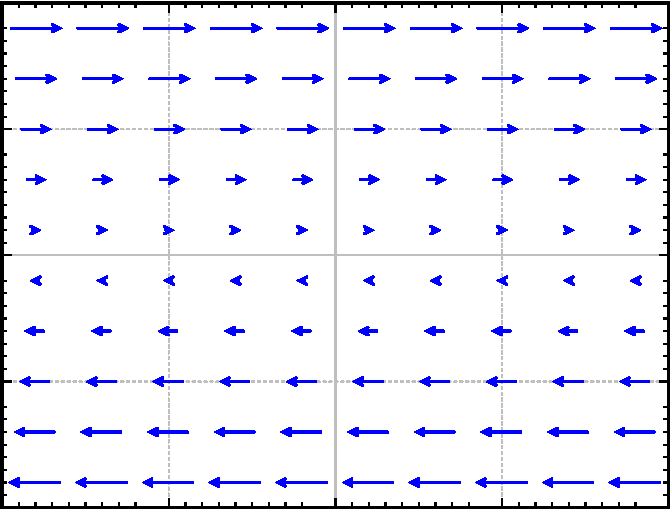
\includegraphics[width=2in]{figures/0100vectorfield}
\\
The solution does not move anywhere if $y = 0$. When $y$ is positive,
the solution moves (with constant speed)
in the positive $x$ direction. When $y$ is
negative, the solution moves (with constant speed) in the negative
$x$ direction. It is not one of the behaviors we have seen.
\\
Note that the matrix has a double eigenvalue 0 and the general solution is
$x = C_1 t + C_2$ and $y = C_1$, which agrees with the
description above.
}

